\documentclass[preprint,12pt,authoryear]{elsarticle}
\usepackage[margin=1in]{geometry}
\usepackage[T1]{fontenc}
\usepackage{lmodern}
\usepackage{microtype}
\usepackage{amsmath,amssymb}
\usepackage{graphicx}
\usepackage{booktabs}
\usepackage{threeparttable}
\usepackage{xcolor}
\usepackage{enumitem}
\usepackage{setspace}
\usepackage[font=small,labelfont=bf]{caption}
\usepackage{tikz}
\usetikzlibrary{arrows.meta,positioning,calc}
\usepackage[colorlinks=true,linkcolor=black,citecolor={blue!55!black},urlcolor={blue!55!black}]{hyperref}
\setlist{nosep,leftmargin=1.4em}
\setstretch{1.15}
\newcommand{\NCompanies}{377}
\newcommand{\NForecasts}{31{,}455}
\newcommand{\NOrigins}{13}
\newcommand{\XsN}{344}
\newcommand{\XsRho}{0.34}
\newcommand{\XsP}{<0.001}
\newcommand{\XsCiLo}{0.23}
\newcommand{\XsCiHi}{0.44}
\newcommand{\XsSevereFragile}{18\%}
\newcommand{\XsSevereRobust}{3\%}
\newcommand{\RevRawNinety}{71\%}
\newcommand{\RevConfNinety}{91\%}
\newcommand{\RevRawFifty}{35\%}
\newcommand{\RevConfFifty}{51\%}
\newcommand{\RevSkill}{28\%}
\newcommand{\RevBeat}{69\%}
\newcommand{\RevRegimeGain}{0.5\%}
\newcommand{\RevN}{15{,}776}
\newcommand{\CashRawNinety}{37\%}
\newcommand{\CashConfNinety}{91\%}
\newcommand{\CashRawFifty}{21\%}
\newcommand{\CashConfFifty}{52\%}
\newcommand{\CashSkill}{-19\%}
\newcommand{\CashBeat}{45\%}
\newcommand{\CashRegimeGain}{0.1\%}
\newcommand{\CashN}{15{,}679}
\newcommand{\NDashboard}{394}
\newcommand{\StructAAPLCovidErr}{-2\%}
\newcommand{\StructAAPLCovidModel}{\$179.1B}
\newcommand{\StructAAPLCovidActual}{\$182.1B}
\newcommand{\StructAAPLCovidCorr}{0.97}
\newcommand{\StructAAPLHikesErr}{-16\%}
\newcommand{\StructAAPLHikesModel}{\$170.7B}
\newcommand{\StructAAPLHikesActual}{\$204.4B}
\newcommand{\StructAAPLHikesCorr}{0.67}
\newcommand{\StructTSLACovidErr}{78\%}
\newcommand{\StructTSLACovidModel}{\$13.9B}
\newcommand{\StructTSLACovidActual}{\$7.8B}
\newcommand{\StructTSLACovidCorr}{0.92}
\newcommand{\StructTSLAHikesErr}{136\%}
\newcommand{\StructTSLAHikesModel}{\$29.8B}
\newcommand{\StructTSLAHikesActual}{\$12.6B}
\newcommand{\StructTSLAHikesCorr}{0.37}
\newcommand{\StructCCLCovidErr}{27\%}
\newcommand{\StructCCLCovidModel}{$-$\$12.8B}
\newcommand{\StructCCLCovidActual}{$-$\$17.6B}
\newcommand{\StructCCLCovidCorr}{0.66}
\newcommand{\StructCCLHikesErr}{645\%}
\newcommand{\StructCCLHikesModel}{\$30.6B}
\newcommand{\StructCCLHikesActual}{$-$\$5.6B}
\newcommand{\StructCCLHikesCorr}{0.55}
\newcommand{\StructBACovidErr}{64\%}
\newcommand{\StructBACovidModel}{$-$\$8.7B}
\newcommand{\StructBACovidActual}{$-$\$24.1B}
\newcommand{\StructBACovidCorr}{0.09}
\newcommand{\StructBAHikesErr}{-247\%}
\newcommand{\StructBAHikesModel}{$-$\$9.9B}
\newcommand{\StructBAHikesActual}{\$6.7B}
\newcommand{\StructBAHikesCorr}{0.66}
\newcommand{\StructINTCCovidErr}{15\%}
\newcommand{\StructINTCCovidModel}{\$37.2B}
\newcommand{\StructINTCCovidActual}{\$32.3B}
\newcommand{\StructINTCCovidCorr}{-0.07}
\newcommand{\StructINTCHikesErr}{187\%}
\newcommand{\StructINTCHikesModel}{\$20.7B}
\newcommand{\StructINTCHikesActual}{$-$\$23.7B}
\newcommand{\StructINTCHikesCorr}{0.31}
\newcommand{\StructNFLXCovidErr}{-308\%}
\newcommand{\StructNFLXCovidModel}{$-$\$3.7B}
\newcommand{\StructNFLXCovidActual}{\$1.8B}
\newcommand{\StructNFLXCovidCorr}{0.22}
\newcommand{\StructNFLXHikesErr}{-66\%}
\newcommand{\StructNFLXHikesModel}{\$2.9B}
\newcommand{\StructNFLXHikesActual}{\$8.5B}
\newcommand{\StructNFLXHikesCorr}{0.69}
\newcommand{\CclBaseHealth}{70}
\newcommand{\CclStressHealth}{12}

% generated by engine/scripts/research_assets.py from research.json
\newcommand{\AttrShare}{75\%}
\newcommand{\AttrShareBk}{15\%}
\newcommand{\AttrShareNonBk}{77\%}
\newcommand{\AttrSixteen}{6.7}
\newcommand{\AttrSixteenIpw}{7.1}
\newcommand{\AttrTwin}{8.1}
\newcommand{\AttrTwinIpw}{8.6}
\newcommand{\AudFirmQuarters}{191{,}189}
\newcommand{\AudFirmsNew}{474}
\newcommand{\AudFirmsOld}{507}
\newcommand{\AudGapsNew}{643}
\newcommand{\AudGapsOld}{943}
\newcommand{\AudLatest}{90\%}
\newcommand{\AudLoaded}{5{,}219}
\newcommand{\AudNoFiling}{91}
\newcommand{\AudRecovered}{37}
\newcommand{\AudUntagged}{552}
\newcommand{\BkFourAltman}{0.85}
\newcommand{\BkFourEv}{224}
\newcommand{\BkFourFormula}{0.90}
\newcommand{\BkFourOhlson}{0.88}
\newcommand{\BkFourTwin}{0.90}
\newcommand{\BkPanAltman}{0.82}
\newcommand{\BkPanEv}{420}
\newcommand{\BkPanFcf}{0.78}
\newcommand{\BkPanFirms}{239}
\newcommand{\BkPanFormula}{0.87}
\newcommand{\BkPanFormulaDiff}{+0.003}
\newcommand{\BkPanFormulaP}{=0.584}
\newcommand{\BkPanN}{21{,}084}
\newcommand{\BkPanOhlson}{0.86}
\newcommand{\BkPanSize}{0.63}
\newcommand{\BkPanTwin}{0.87}
\newcommand{\BkTwentyAltman}{0.81}
\newcommand{\BkTwentyEv}{52}
\newcommand{\BkTwentyFcf}{0.77}
\newcommand{\BkTwentyFormula}{0.87}
\newcommand{\BkTwentyFormulaDiff}{+0.005}
\newcommand{\BkTwentyFormulaP}{=0.737}
\newcommand{\BkTwentyN}{2{,}015}
\newcommand{\BkTwentyOhlson}{0.79}
\newcommand{\BkTwentySize}{0.57}
\newcommand{\BkTwentyTwin}{0.87}
\newcommand{\BkTwentyWeakAltman}{0.64}
\newcommand{\BkTwentyWeakFcf}{0.52}
\newcommand{\BkTwentyWeakFormula}{0.76}
\newcommand{\BkTwentyWeakFormulaDiff}{+0.012}
\newcommand{\BkTwentyWeakFormulaP}{=0.724}
\newcommand{\BkTwentyWeakOhlson}{0.73}
\newcommand{\BkTwentyWeakSize}{0.42}
\newcommand{\BkTwentyWeakTwin}{0.77}
\newcommand{\BkWeakAltman}{0.66}
\newcommand{\BkWeakEv}{335}
\newcommand{\BkWeakFcf}{0.58}
\newcommand{\BkWeakFormula}{0.77}
\newcommand{\BkWeakFormulaDiff}{+0.022}
\newcommand{\BkWeakFormulaP}{=0.012}
\newcommand{\BkWeakN}{6{,}749}
\newcommand{\BkWeakOhlson}{0.77}
\newcommand{\BkWeakShare}{80\%}
\newcommand{\BkWeakSize}{0.52}
\newcommand{\BkWeakTwin}{0.79}
\newcommand{\CalAciCash}{91\%}
\newcommand{\CalAciCashOk}{misses}
\newcommand{\CalAciCashStress}{89\%}
\newcommand{\CalAciRev}{91\%}
\newcommand{\CalAciRevOk}{misses}
\newcommand{\CalAciRevStress}{78\%}
\newcommand{\CalCashBelow}{35\%}
\newcommand{\CalCashConf}{91\%}
\newcommand{\CalCashErrSizeT}{$-$8.5}
\newcommand{\CalCashRaw}{39\%}
\newcommand{\CalCashStress}{89\%}
\newcommand{\CalCashWidthSizeT}{1.1}
\newcommand{\CalCondCash}{91\%}
\newcommand{\CalCondCashOk}{misses}
\newcommand{\CalCondCashStress}{88\%}
\newcommand{\CalCondRev}{90\%}
\newcommand{\CalCondRevOk}{misses}
\newcommand{\CalCondRevStress}{79\%}
\newcommand{\CalRevBelow}{13\%}
\newcommand{\CalRevConf}{91\%}
\newcommand{\CalRevRaw}{78\%}
\newcommand{\CalRevStress}{78\%}
\newcommand{\CalRevYearMin}{78\%}
\newcommand{\CashHybHi}{1.3\%}
\newcommand{\CashHybLo}{0.0\%}
\newcommand{\CashHybSkill}{0.7\%}
\newcommand{\CashHybVerdict}{meets}
\newcommand{\CashLamHi}{0.20}
\newcommand{\CashLamLo}{0.15}
\newcommand{\CensusFound}{33}
\newcommand{\CensusLegacy}{35}
\newcommand{\CensusMissing}{CEC Entertainment and Hornbeck Offshore Services}
\newcommand{\CensusRepeat}{63\%}
\newcommand{\CovAllAbnFcf}{$-$0.14}
\newcommand{\CovAllAbnRevVol}{0.01}
\newcommand{\CovAllAbnTwin}{0.04}
\newcommand{\CovAllAltman}{0.28}
\newcommand{\CovAllFcf}{0.66}
\newcommand{\CovAllFormula}{0.34}
\newcommand{\CovAllN}{1{,}651}
\newcommand{\CovAllTwin}{0.33}
\newcommand{\CovEdgarN}{2{,}035}
\newcommand{\CovSpAbnFcf}{0.09}
\newcommand{\CovSpAbnRevVol}{0.08}
\newcommand{\CovSpAbnTwin}{0.16}
\newcommand{\CovSpAltman}{0.37}
\newcommand{\CovSpFcf}{0.83}
\newcommand{\CovSpFormula}{0.34}
\newcommand{\CovSpN}{341}
\newcommand{\CovSpTodayTwin}{0.35}
\newcommand{\CovSpTwin}{0.34}
\newcommand{\DecCapexDelta}{0.033}
\newcommand{\DecCapexNoBone}{0.61}
\newcommand{\DecCapexStatic}{0.65}
\newcommand{\DecCapexTwin}{0.64}
\newcommand{\DecCashDelta}{0.009}
\newcommand{\DecCashNoRtwo}{0.50}
\newcommand{\DecCashTwin}{0.55}
\newcommand{\DecDebtDelta}{0.022}
\newcommand{\DecDivDelta}{0.008}
\newcommand{\ElastCapexRatio}{0.94}
\newcommand{\ElastCfoRatio}{0.7}
\newcommand{\ElastCfoReal}{0.28}
\newcommand{\ElastCfoTwin}{0.19}
\newcommand{\ElastEbitdaRatio}{0.6}
\newcommand{\EpiFifteenClusters}{52}
\newcommand{\EpiFifteenDepth}{9\%}
\newcommand{\EpiFifteenFormulaT}{$-$1.2}
\newcommand{\EpiFifteenT}{2.3}
\newcommand{\EpiFifteenTRobust}{2.04}
\newcommand{\EpiTwentyClusters}{54}
\newcommand{\EpiTwentyDepth}{18\%}
\newcommand{\EpiTwentyFormulaT}{$-$1.9}
\newcommand{\EpiTwentyT}{3.5}
\newcommand{\EpiTwentyTRobust}{4.04}
\newcommand{\EpiTwentyTwoClusters}{55}
\newcommand{\EpiTwentyTwoDepth}{8\%}
\newcommand{\EpiTwentyTwoFormulaT}{$-$3.9}
\newcommand{\EpiTwentyTwoT}{3.9}
\newcommand{\EpiTwentyTwoTRobust}{4.60}
\newcommand{\EpiVerdict}{generalizes}
\newcommand{\ExAmznReal}{40\%}
\newcommand{\ExAmznRev}{53\%}
\newcommand{\ExAmznRule}{39\%}
\newcommand{\ExAmznTwin}{44\%}
\newcommand{\ExFordReal}{26\%}
\newcommand{\ExFordRev}{$-$15\%}
\newcommand{\ExFordRule}{19\%}
\newcommand{\ExFordTwin}{15\%}
\newcommand{\ExGeReal}{7\%}
\newcommand{\ExGeRev}{$-$33\%}
\newcommand{\ExGeRule}{29\%}
\newcommand{\ExGeTwin}{34\%}
\newcommand{\ExGmReal}{23\%}
\newcommand{\ExGmRev}{$-$19\%}
\newcommand{\ExGmRule}{18\%}
\newcommand{\ExGmTwin}{10\%}
\newcommand{\ExRightSign}{62\%}
\newcommand{\ExpDepth}{17\%}
\newcommand{\ExpFcfAbnT}{$-$4.0}
\newcommand{\ExpFormulaAbnT}{$-$0.3}
\newcommand{\ExpOnlyAbn}{0.09}
\newcommand{\ExpTwinAbn}{0.04}
\newcommand{\ExpTwinAbnT}{1.9}
\newcommand{\ExpTwinRaw}{0.37}
\newcommand{\ExpUniformRaw}{0.33}
\newcommand{\FcCashEts}{$-$35\%}
\newcommand{\FcCashRw}{$-$27\%}
\newcommand{\FcFirms}{470}
\newcommand{\FcRevEts}{20\%}
\newcommand{\FcRevEtsT}{$-$3.67}
\newcommand{\FcRevN}{18{,}768}
\newcommand{\FcRevRw}{28\%}
\newcommand{\FcRevRwT}{$-$5.41}
\newcommand{\FcfCapexShare}{6\%}
\newcommand{\FcfGainCapex}{0.01}
\newcommand{\FcfGainCfo}{0.11}
\newcommand{\FcfGainFcf}{0.20}
\newcommand{\HOneVerdict}{rejected}
\newcommand{\HThreeVerdict}{accepted}
\newcommand{\HThreeWins}{3}
\newcommand{\HetDownN}{2{,}716}
\newcommand{\HetDownSixteen}{0.31}
\newcommand{\HetDownTwin}{0.27}
\newcommand{\HetLevHighTwinReg}{0.44}
\newcommand{\HetLevLowTwinReg}{0.53}
\newcommand{\NBench}{13}
\newcommand{\PanAbnTwinAuc}{0.54}
\newcommand{\PanFcfAuc}{0.82}
\newcommand{\PanFirmYears}{21{,}171}
\newcommand{\PanFirms}{3{,}435}
\newcommand{\PanOosDelta}{+0.004}
\newcommand{\PanOosYears}{2017--2024}
\newcommand{\PanTwinAuc}{0.76}
\newcommand{\RevAccepted}{accepted}
\newcommand{\RevAucBase}{0.806}
\newcommand{\RevAucNew}{0.811}
\newcommand{\RevDiff}{0.1}
\newcommand{\RevDiffHi}{0.1}
\newcommand{\RevDiffLo}{0.0}
\newcommand{\RevFirstYear}{2018}
\newcommand{\RevFive}{8.0}
\newcommand{\RevIndAuc}{0.810}
\newcommand{\RevIndMae}{8.6}
\newcommand{\RevMaeBase}{8.7}
\newcommand{\RevMaeNew}{8.6}
\newcommand{\RevNone}{8.1}
\newcommand{\RevTestN}{10{,}905}
\newcommand{\SensBkHi}{0.82}
\newcommand{\SensBkLo}{0.81}
\newcommand{\SensIncrHi}{0.39}
\newcommand{\SensIncrLo}{0.38}
\newcommand{\SensMaeHigh}{8.2}
\newcommand{\SensMaeLow}{8.0}
\newcommand{\SmallAucFormula}{0.71}
\newcommand{\SmallAucTwin}{0.72}
\newcommand{\SmallBk}{19}
\newcommand{\SmallFirms}{381}
\newcommand{\SmallIncr}{0.32}
\newcommand{\SmallMaeSixteen}{30.5}
\newcommand{\SmallMaeTwin}{35.8}
\newcommand{\SmallN}{1{,}158}
\newcommand{\SobIncrMax}{0.45}
\newcommand{\SobIncrMin}{0.31}
\newcommand{\SobMaeMax}{11.6}
\newcommand{\SobMaeMin}{7.6}
\newcommand{\SobN}{311}
\newcommand{\SobPoints}{2560}
\newcommand{\SobRestST}{0.56}
\newcommand{\SobSpecIncr}{0.41}
\newcommand{\SobSpecMae}{8.4}
\newcommand{\SobTopLabel}{prior s.d. (tau)}
\newcommand{\SobTopST}{0.70}
\newcommand{\TimCashDiff}{0.04}
\newcommand{\TimCashDiffHi}{0.05}
\newcommand{\TimCashDiffLo}{0.03}
\newcommand{\TimCashNoLoops}{0.50}
\newcommand{\TimCashStatic}{0.52}
\newcommand{\TimCashTwin}{0.54}
\newcommand{\TimDebtNoLoops}{0.58}
\newcommand{\TimDebtTwin}{0.58}
\newcommand{\TrEncFcfTwinT}{9.4}
\newcommand{\TrEncLevFcfTwinT}{8.4}
\newcommand{\TrEncLevTwinCoef}{0.21}
\newcommand{\TrEncLevTwinT}{7.6}
\newcommand{\TrEncLevelsTwinTTwoWay}{8.8}
\newcommand{\TrEncRegT}{9.7}
\newcommand{\TrEncShrunkT}{5.6}
\newcommand{\TrEncShrunkTTwoWay}{4.2}
\newcommand{\TrEncSixteenT}{8.8}
\newcommand{\TrEncTwinCoef}{0.23}
\newcommand{\TrEncTwinT}{8.5}
\newcommand{\TrEncTwinTTwoWay}{8.4}
\newcommand{\TrFcfHybGainPct}{3.7\%}
\newcommand{\TrFcfTwinVsSixteen}{0.23}
\newcommand{\TrFcfVsBestNull}{0.20}
\newcommand{\TrFcfVsBestNullHi}{0.37}
\newcommand{\TrFcfVsBestNullLo}{0.02}
\newcommand{\TrFcfVsBestNullP}{=0.036}
\newcommand{\TrFcfVsWorstP}{=0.040}
\newcommand{\TrFirms}{2{,}602}
\newcommand{\TrFourVsSixteen}{0.21}
\newcommand{\TrHlnRegOverTwin}{9.5}
\newcommand{\TrHlnSixteenOverTwin}{8.9}
\newcommand{\TrHlnTwinOverReg}{6.0}
\newcommand{\TrHlnTwinOverSixteen}{6.2}
\newcommand{\TrHybDollar}{46}
\newcommand{\TrHybGain}{0.46}
\newcommand{\TrHybGainHi}{0.63}
\newcommand{\TrHybGainLo}{0.29}
\newcommand{\TrHybGainPct}{3.6\%}
\newcommand{\TrHybN}{11{,}274}
\newcommand{\TrHybRegFiveGainPct}{2.8\%}
\newcommand{\TrHybSixteen}{12.84}
\newcommand{\TrHybSixteenReg}{12.52}
\newcommand{\TrHybSixteenRegFive}{12.49}
\newcommand{\TrHybSixteenTwin}{12.37}
\newcommand{\TrHybTwin}{14.80}
\newcommand{\TrHybVsFour}{0.27}
\newcommand{\TrHybVsFourP}{=0.012}
\newcommand{\TrHybVsNull}{0.14}
\newcommand{\TrHybVsNullP}{=0.088}
\newcommand{\TrHybVsRegFive}{0.11}
\newcommand{\TrHybVsRegFiveP}{=0.180}
\newcommand{\TrIncrEight}{0.31}
\newcommand{\TrIncrReg}{0.25}
\newcommand{\TrIncrShrunk}{0.14}
\newcommand{\TrIncrSixteen}{0.40}
\newcommand{\TrIncrSixteenHi}{0.42}
\newcommand{\TrIncrSixteenLo}{0.38}
\newcommand{\TrIncrTwin}{0.38}
\newcommand{\TrIncrTwinHi}{0.40}
\newcommand{\TrIncrTwinLo}{0.36}
\newcommand{\TrLambdaHi}{0.20}
\newcommand{\TrLambdaLo}{0.15}
\newcommand{\TrMaeNfive}{9.0}
\newcommand{\TrMaeNfour}{7.9}
\newcommand{\TrMaeNone}{7.5}
\newcommand{\TrMaeNsix}{9.0}
\newcommand{\TrMaeNthree}{6.7}
\newcommand{\TrMaeNtwo}{7.1}
\newcommand{\TrMaeTone}{8.1}
\newcommand{\TrMaeTzero}{8.2}
\newcommand{\TrN}{15{,}933}
\newcommand{\TrNRound}{16{,}000}
\newcommand{\TrTwinVsReg}{0.50}
\newcommand{\TrTwinVsRegHi}{0.51}
\newcommand{\TrTwinVsRegLo}{0.48}
\newcommand{\TrTwinVsShrunk}{0.41}
\newcommand{\TrTwinVsShrunkHi}{0.43}
\newcommand{\TrTwinVsShrunkLo}{0.40}
\newcommand{\TrTwinVsSixteen}{0.23}
\newcommand{\TrTwinVsSixteenHi}{0.25}
\newcommand{\TrTwinVsSixteenLo}{0.21}
\newcommand{\TrVerdict}{survives}
\newcommand{\TwoWayHi}{0.26}
\newcommand{\TwoWayLo}{0.19}
\newcommand{\UniverseBk}{475}
\newcommand{\UniverseN}{5{,}309}

% generated by engine/scripts/rev3_assets.py from research.json and rev3/inputs.json
\newcommand{\BkAucTwin}{0.87}
\newcommand{\BkAucZ}{0.82}
\newcommand{\CeAucTwin}{0.66}
\newcommand{\CeAucZ}{0.64}
\newcommand{\CeEv}{1{,}539}
\newcommand{\CrpsVthree}{207}
\newcommand{\CrpsVthreedef}{132}
\newcommand{\CrpsVtwopre}{26}
\newcommand{\CrpsVtworev}{24}
\newcommand{\DenBetterEmp}{2}
\newcommand{\DenBetterGauss}{6}
\newcommand{\DenCov}{30\%}
\newcommand{\DenCovFcf}{28\%}
\newcommand{\DenCrpsEmp}{29}
\newcommand{\DenCrpsGauss}{110}
\newcommand{\DenCrpsTwin}{207}
\newcommand{\DenN}{11{,}274}
\newcommand{\DenPitEmpTails}{30\%}
\newcommand{\DenPitHigh}{35\%}
\newcommand{\DenPitLow}{42\%}
\newcommand{\DenPitTails}{77\%}
\newcommand{\DenWorstDiff}{1255}
\newcommand{\DenWorstYear}{2021}
\newcommand{\DenYears}{8}
\newcommand{\DmAbsP}{0.329}
\newcommand{\DmAbsT}{1.03}
\newcommand{\ElastRatioExact}{0.67}
\newcommand{\ElastVerdict}{outside}
\newcommand{\ElastVthree}{0.67}
\newcommand{\ElastVthreedef}{0.88}
\newcommand{\ElastVtwopre}{2.18}
\newcommand{\ElastVtworev}{1.24}
\newcommand{\EncAbsReg}{1.15}
\newcommand{\EncAbsSixteen}{$-$0.86}
\newcommand{\EncAbsSixteenP}{0.794}
\newcommand{\EncLadCoef}{0.000}
\newcommand{\EncLadRegT}{3.73}
\newcommand{\EncLadT}{0.00}
\newcommand{\EncTGOne}{7.3}
\newcommand{\EncTGOneCrit}{2.23}
\newcommand{\EncTGOnePsd}{not positive semi-definite}
\newcommand{\FamB}{10{,}000}
\newcommand{\FamCombMeanDiff}{$-$0.38}
\newcommand{\FamCombMeanRw}{0.021}
\newcommand{\FamCombMedDiff}{$-$0.20}
\newcommand{\FamCombMedRw}{0.370}
\newcommand{\FamCombRejects}{2}
\newcommand{\FamRegMeanRw}{0.020}
\newcommand{\FamRejects}{8}
\newcommand{\FamTwinMedDiff}{1.27}
\newcommand{\FamTwinMedRw}{0.004}
\newcommand{\GainDmP}{$<$0.001}
\newcommand{\GainFcfPct}{3.5\%}
\newcommand{\GainFourHi}{6.0\%}
\newcommand{\GainFourLo}{$-$2.1\%}
\newcommand{\GainFourPct}{2.4\%}
\newcommand{\GainFourPos}{5}
\newcommand{\GainHi}{4.1\%}
\newcommand{\GainLo}{2.4\%}
\newcommand{\GainLoopsPct}{0.33\%}
\newcommand{\GainPct}{3.3\%}
\newcommand{\GainPos}{8}
\newcommand{\GainRegHi}{1.9\%}
\newcommand{\GainRegLo}{0.5\%}
\newcommand{\GainRegPct}{1.2\%}
\newcommand{\GainYears}{8}
\newcommand{\LadFive}{10.5}
\newcommand{\LadLegacy}{11.7}
\newcommand{\LadLegacyN}{3{,}216}
\newcommand{\LadN}{2{,}981}
\newcommand{\LadOne}{8.9}
\newcommand{\LadPre}{11.4}
\newcommand{\LadThree}{8.3}
\newcommand{\LamMax}{0.25}
\newcommand{\LamMin}{0.20}
\newcommand{\LockDigest}{65e0f04e5905}
\newcommand{\MaeVthree}{8.1}
\newcommand{\MaeVthreedef}{8.1}
\newcommand{\MaeVtwopre}{11.1}
\newcommand{\MaeVtworev}{8.8}
\newcommand{\McsCombP}{1.000}
\newcommand{\McsSize}{10}
\newcommand{\McsTwinIn}{excludes}
\newcommand{\McsTwinP}{0.006}
\newcommand{\RivAucAll}{0.87}
\newcommand{\RivAucBench}{0.86}
\newcommand{\RivAucNonacc}{0.63}
\newcommand{\RivAucTwin}{0.87}
\newcommand{\RivEv}{285}
\newcommand{\RivN}{14{,}257}
\newcommand{\RivTwinBeyond}{0.026}
\newcommand{\RivTwinBeyondHi}{0.037}
\newcommand{\RivTwinBeyondLo}{0.016}
\newcommand{\SOneBlockHi}{$-$2.28}
\newcommand{\SOneBlockLo}{$-$3.75}
\newcommand{\SOneContStat}{$-$3.06}
\newcommand{\SOneDefStat}{$-$2.98}
\newcommand{\SOneDmMean}{126.8}
\newcommand{\SOneDmP}{0.32}
\newcommand{\SOneFamStat}{$-$3.01}
\newcommand{\SOneFamVerdict}{succeeds}
\newcommand{\SOneG}{11}
\newcommand{\SOneHi}{$-$2.15}
\newcommand{\SOneLo}{$-$3.76}
\newcommand{\SOneLost}{1}
\newcommand{\SOneMean}{$-$2.95}
\newcommand{\SOneMedVthree}{8.09}
\newcommand{\SOneMedVtwo}{11.10}
\newcommand{\SOneN}{15{,}932}
\newcommand{\SOneNeg}{11}
\newcommand{\SOneStat}{$-$3.01}
\newcommand{\SOneVerdict}{succeeds}
\newcommand{\SelLamMax}{0.5}
\newcommand{\SelLamMin}{0.3}
\newcommand{\SelTauFirst}{$\infty$}
\newcommand{\SelTauMode}{0.50}
\newcommand{\SelYears}{2018--2024}
\newcommand{\ShortBase}{15.2\%}
\newcommand{\ShortBrierLogit}{0.127}
\newcommand{\ShortBrierTwin}{0.152}
\newcommand{\ShortBss}{$-$0.20}
\newcommand{\ShortBssHi}{$-$0.17}
\newcommand{\ShortBssLo}{$-$0.22}
\newcommand{\ShortEv}{1{,}344}
\newcommand{\ShortExcluded}{64}
\newcommand{\ShortLowBinRate}{13.9\%}
\newcommand{\ShortLowBinShare}{93\%}
\newcommand{\ShortMeanP}{4.1\%}
\newcommand{\ShortN}{8{,}818}
\newcommand{\ShortRel}{0.026}
\newcommand{\ShortRes}{0.003}
\newcommand{\ShortResLogit}{0.003}
\newcommand{\ShortVerdict}{fails}
\newcommand{\SnapDigest}{f0f6e091b610da1d}
\newcommand{\SpaCfoMean}{0.002}
\newcommand{\SpaCfoMed}{0.059}
\newcommand{\SpaFcfMean}{0.003}
\newcommand{\SpaFcfMed}{0.310}
\newcommand{\SpecN}{15{,}933}

\newcommand{\twin}{FinTwin}
\journal{International Journal of Forecasting}

\begin{document}
\begin{frontmatter}
\title{Does Filing-Based Cash-Flow Simulation Beat Persistence?\\A Pre-Registered Benchmark on a Survivorship-Free Panel of SEC Filers}
\author{Spilios Dimakopoulos}
\ead{spiliosdimakk@gmail.com}
\address{Independent researcher. Code and data: \url{https://github.com/SpiliosDimakopoulos/fintwin}, archived at \href{https://doi.org/10.5281/zenodo.23434606}{doi:10.5281/zenodo.23434606}.}

\begin{abstract}
\noindent Simulation models of the firm promise conditional forecasts: how a given revenue path turns into cash, and how likely a liquidity shortfall is under a stated shock. We test whether such a model forecasts better than persistence. \twin{} is a stock-and-flow model calibrated for each firm from point-in-time SEC XBRL filings. On a survivorship-free universe of \UniverseN{} non-financial filers (2014--2024) and a frozen data snapshot, we report three specifications side by side and evaluate them under rules fixed before the runs. Pillar A asks whether, given the realized revenue path, the simulated eight-quarter operating cash flow is informative beyond simple rules. Correcting implementation errors lowers the median error from \SOneMedVtwo{} to \SOneMedVthree{} percentage points of revenue (all \SOneNeg{} years improve; the pre-specified test succeeds), but the corrected model is still less accurate than a 16-quarter cash-flow margin (\TrMaeNthree), and its response to revenue is now too weak (\ElastRatioExact{} times the realized one, outside the pre-specified range). Its departures from the margin remain significant in squared-loss encompassing regressions but not under absolute loss, and adding about a fifth of them to the margin lowers the mean absolute error by \GainPct{}, a gain that a simple regression rule shares in part. Pillar B asks whether the simulator's distributions and stress probabilities are useful. They are not: its predictive distributions are far too narrow (a 90\% interval covers \DenCov{} of outcomes) and its CRPS is not better than that of a Gaussian or empirical residual distribution; its probability of a liquidity shortfall under a recession scenario has a Brier skill of \ShortBss{} against a logit on three opening ratios. As a ranking device it is competitive with accounting scores (bankruptcy AUC \BkAucTwin). Filing-based simulation mostly encodes persistence; what it adds is a small, mean-loss improvement to point forecasts, not calibrated uncertainty.
\end{abstract}

\begin{keyword}
forecast evaluation \sep pre-registration \sep cash-flow forecasting \sep density forecasts \sep stress testing \sep forecast encompassing \sep corporate liquidity \sep XBRL
\JEL C53 \sep G17 \sep G32 \sep G33 \sep M41
\end{keyword}
\end{frontmatter}

\section{Introduction}\label{sec:intro}

A corporate stress test asks a conditional question: \emph{if} revenue falls by a third for a year and debt markets close, does the company run out of cash, and when? Credit analysts usually answer it with ratios or accounting distress scores \citep{beaver1966,altman1968,ohlson1980,zmijewski1984}. A simulation model promises more. It represents the mechanisms through which a shock becomes a cash shortfall (fixed costs, working capital, maturing debt, credit lines, the loss of market access) and runs them forward over many paths, so that it gives both a point forecast and a distribution. System dynamics provides the language for such models \citep{forrester1961,sterman2000}; engineering calls a simulation kept synchronized with its physical counterpart a digital twin \citep{grieves2017,tao2019,kritzinger2018}.

This paper asks whether such a model forecasts better than persistence, and treats the question as a forecasting benchmark with pre-specified rules. The model, \twin{}, is calibrated for each company from its own point-in-time XBRL filings and is open source. Earlier versions of this paper found that its apparent skill came mostly from persistence: a statistic that seemed to show information beyond a four-quarter margin rule was matched by a 16-quarter margin with no simulation at all, because profitability mean-reverts \citep{fama2000}. A review of the code then found implementation errors in the cost model, the cash-flow residual, the shock process and the data layer. Correcting errors after seeing results invites the suspicion of tuning. We therefore wrote the corrections and the decision rules for this revision into the repository before changing any code or running any test, ran all specifications on one frozen data snapshot, and report the old and the corrected specifications side by side.

The evaluation has two pillars. \emph{Pillar A} is point transmission. Each model is given the revenue the company actually reported over the eight quarters after a cutoff and predicts cumulative operating cash flow; the rivals are six simple rules that see the same revenue. This isolates how a revenue path becomes cash from the scenario, which no filing can predict. \emph{Pillar B} is distribution and stress. A simulator is built to say how uncertain the outcome is and how likely a shortfall is, so we score its predictive distributions with the CRPS and probability integral transforms and its shortfall probabilities with the Brier score and its decomposition, against statistical rivals estimated on the same earlier years.

The results separate the two pillars. In pillar A the corrections work as intended on their own terms: the median error falls from \SOneMedVtwo{} to \SOneMedVthree{} percentage points of revenue, in every one of \SOneNeg{} years, and the pre-specified test succeeds. They do not make the simulator better than persistence. A 16-quarter margin is still more accurate (\TrMaeNthree), and the corrected model now responds too weakly to revenue, the opposite of the earlier overreaction. Its departures from the margin keep a significant coefficient in squared-loss encompassing regressions, so by the decision rule of the second version the transmission hypothesis still survives; but the information disappears under absolute loss, and out of sample it is worth a mean-absolute-error gain of about \GainPct{} when a fifth of the departure is added to the margin. In pillar B the simulator fails both pre-specified tests. Its predictive distributions of eight-quarter cash flow are far too narrow, and its probability of a liquidity shortfall is worse in Brier score than a logit on three opening ratios, mainly because it assigns near-zero probabilities to most firms that do suffer a shortfall. As a ranking device, by contrast, its scores are competitive with accounting distress scores.

The paper makes three contributions. First, it is an example of a pre-registered benchmark of a structural model against persistence, with a ladder of simple rivals, encompassing tests under two losses, combinations with year-by-year weights, and a family of comparisons controlled with \citet{romano2005}, the model confidence set \citep{hansen2011} and a test for superior predictive ability \citep{hansen2005}. The reporting rule that every specification and every failure is shown, including the corrections that worked on their own terms but did not change the conclusion, is itself part of the evidence. Second, it provides an open, survivorship-free, point-in-time panel of all non-financial XBRL filers with a census of bankruptcy petitions and a frozen snapshot, on which other fundamental models can be tested without hindsight. Third, it gives a measured answer to what a filing-based simulator is for: scenario arithmetic around a persistence forecast, not calibrated uncertainty or early warning.

Section~\ref{sec:framework} relates the simulator to other models of corporate fragility and states the hypotheses. Sections~\ref{sec:data} and~\ref{sec:model} describe the data, the model and the three specifications. Section~\ref{sec:design} sets out the pre-specification and the tests. Sections~\ref{sec:pillarA} and~\ref{sec:pillarB} report the two pillars, Section~\ref{sec:secondary} the secondary evidence, and Section~\ref{sec:discussion} discusses what the results mean and what they do not cover. An online appendix contains the material of the second version that is now secondary: the sensitivity analysis, conformal recalibration, forecasts of revenue and cash for S\&P~500 members, the 2020 cross-section and the downturn decompositions.

\section{Conceptual framework}\label{sec:framework}

\subsection{Twin, shadow or simulation model?}
The term \emph{digital twin} is used loosely, so we state which of its defining properties the model has. \citet{kritzinger2018} separate three levels by the direction and automation of data flows between a physical system and its virtual counterpart: a \emph{digital model} is updated by hand, a \emph{digital shadow} is updated automatically from the physical system, and a \emph{digital twin} also feeds decisions back into the physical system automatically. By this taxonomy \twin{} is a digital shadow with a human in the loop. It is synchronized automatically: every week a scheduled job reads each company's newest filings, re-estimates every parameter and re-runs the simulations, and its state can be rewound to any past filing date. It represents the firm's financial system as stocks and flows that map one-to-one onto the balance sheet, rather than as a statistical summary of it. It also supports decisions through what-if analysis: scenarios, management levers (cutting capital expenditure or payouts, drawing the revolver, issuing debt or equity) and reverse stress tests. It does not close the loop automatically, since no decision taken in the model is executed in the firm. Its synchronization frequency is bounded by the quarterly reporting cycle. We keep the term because the system-dynamics and engineering literature uses it for models with these properties, and because organizational twins are increasingly discussed in management \citep{lyytinen2024}. The evidence in this paper, however, concerns the model, not the label.

\subsection{Relation to existing models}
Table~\ref{tab:framework} places the twin among four families of models that address related questions.

\emph{Accounting-based distress scores} \citep{beaver1966,altman1968,ohlson1980,zmijewski1984} and their hazard-model successors \citep{shumway2001,chava2004,campbell2008} map ratios to the probability of an event. They are estimated on default samples and are not conditional on a scenario. \emph{Structural credit models} \citep{merton1974,leland1994} derive default probabilities from asset value and volatility, inferred from equity prices. Their state variable is a single asset value, not cash, working capital or a maturity ladder, so they cannot say whether a given revenue path exhausts liquidity before the debt is due. \emph{Corporate financial-planning models} \citep{carleton1970,warren1971} are simultaneous-equation projections of the financial statements under managerial assumptions. They are close in spirit to the twin's accounting core but are deterministic, specified by the analyst and rarely validated out of sample. \emph{Top-down corporate stress tests} run by central banks, the IMF and the OECD \citep{imf2020,roulet2020} apply macroeconomic and sector-level scenarios to firm-level data. They project income, funding needs and debt service under common assumptions, without firm-specific feedback between financing conditions and operations. Machine-learning classifiers \citep{barboza2017,mai2019,jones2017} raise the accuracy of distress prediction but, like the scores, are not conditional on a scenario. Finally, the accounting literature on \emph{cash-flow prediction} \citep{dechow1998,barth2001,kim2005,lev2010,nallareddy2020}, on cross-sectional forecasts of earnings \citep{hou2012,li2014} and on the mean reversion of profitability \citep{fama2000} provides the simplest rivals for the twin's transmission mechanics: rules that map revenue or earnings into cash through margins, accruals and working capital.

``Digital twins'' of firms or of the financial system appear in practitioner and early-stage work \citep{westphal2024,anshari2022,bhatia2026}, none of which tests a firm-level twin against simple rivals out of sample. The twin combines elements that these families keep apart: an accounting identity that holds on every path, firm-specific parameters estimated automatically from filings, contractual debt maturities and credit lines, path-dependent financing constraints (feedback loops), and a probabilistic description of uncertainty. Whether this combination predicts anything that the simpler members of each family do not is an empirical question. The rest of the paper answers it against the strongest simple rival in each case.

\begin{table}[t]
\centering\scriptsize
\setlength{\tabcolsep}{3pt}
\caption{Models of corporate financial fragility}
\label{tab:framework}
\begin{tabular}{p{0.2\linewidth}p{0.14\linewidth}p{0.14\linewidth}p{0.14\linewidth}p{0.14\linewidth}p{0.14\linewidth}}
\toprule
 & Distress scores & Structural credit & Financial planning & Top-down stress tests & \twin{} \\
\midrule
Question & probability of default & default probability from market values & projected statements & sector shock $\rightarrow$ firm losses & shock path $\rightarrow$ cash, debt, breaches \\
Conditional on a scenario & no & partly & yes & yes & yes \\
State variables & ratios & asset value & statements & balance sheet & 9 balance-sheet stocks \\
Liquidity timing (maturities, credit lines) & no & no & sometimes & sometimes & yes \\
Feedback (spreads, market access, management response) & no & endogenous default & no & rarely & 4 loops \\
Uncertainty & event probability & diffusion & none & scenarios & Monte Carlo \\
Parameters & pooled estimates & market-implied & analyst & mixed & per firm, from filings \\
Updating & periodic re-estimation & daily & manual & annual & weekly, automatic \\
\bottomrule
\end{tabular}
\end{table}

\subsection{Further related work}
\paragraph{Corporate liquidity.} Firms hold cash and credit lines to insure against cash-flow shortfalls \citep{opler1999,almeida2004,bates2009,sufi2009}. The 2020 shock offered a natural experiment. \citet{fahlenbrach2021} show that firms with more financial flexibility before the pandemic suffered smaller stock-price declines, \citet{ramelli2020} and \citet{ding2021} document that pre-pandemic leverage and cash holdings shaped stock returns, and \citet{acharya2020} describe the dash for cash through credit-line drawdowns and bond issuance by firms at risk of downgrade. These studies explain market reactions with balance-sheet characteristics. We use the same episode to evaluate a model that was not estimated on it, and we measure outcomes in cash rather than in prices.

\paragraph{Forecast evaluation.} We evaluate the twin's predictive distributions with the continuous ranked probability score and probability integral transform histograms \citep{gneiting2007,gneiting2007b}, compare predictive accuracy with Diebold--Mariano tests \citep{diebold1995} and test forecast encompassing \citep{harvey1998,clark2001,giacomini2006} using clustered standard errors \citep{petersen2009,cameron2008}, benchmark against exponential smoothing in state-space form \citep{hyndman2008}, and recalibrate intervals with online split-conformal prediction \citep{vovk2005,gibbs2021}. Combinations of forecasts are evaluated against the evidence that simple averages are hard to beat \citep{bates1969,clemen1989,timmermann2006,claeskens2016}.


\subsection{Hypotheses}
The design of Section~\ref{sec:design} tests three hypotheses, each against rivals that see the same information.

\begin{description}
\item[H1 (ranking).] Under a common scenario, the twin's stress score ranks firms' subsequent distress better than accounting scores and simple cash-flow benchmarks computed from the same filings.
\item[H2 (transmission).] Given the revenue path that actually occurred, the twin's cash-flow response contains information about realized cash flows that is not contained in margin rules (including long-window and industry-shrunk margins) or in a per-firm regression of cash flow on revenue and its change.
\item[H3 (feedback).] The feedback loops improve the prediction of the outcomes they are designed to produce --- new borrowing, cash depletion, dividend and capital-expenditure cuts --- not only the cross-sectional ranking of firms.
\end{description}

\noindent Only the H2 rule was fixed before any result was seen. Rules for H1 and H3 were written later, after the first round's bankruptcy and loop results had been computed, so their evaluations are descriptive, not confirmatory. H2 is accepted only if the twin's incremental correlation against each of the 16-quarter margin, the industry-shrunk margin and the regression with revenue timing has a confidence interval above zero and its coefficient in an encompassing regression \citep{chong1986,fair1990} is significant at 5\%.


\section{Data}\label{sec:data}

All runs in this paper read one frozen copy of the EDGAR, FRED and real-time GDP inputs (digest \texttt{\SnapDigest}), so that differences between specifications come from the code alone. The snapshot is archived with the code.

\subsection{Point-in-time XBRL panels}
The SEC \texttt{companyfacts} endpoint returns every value a registrant has tagged in XBRL since 2009, with the period it describes, the form, the filing date and the accession number. We build a quarterly panel of 38 fields per company from 72 tags (income statement, cash-flow statement, balance sheet, debt by component, impairments, customer deposits and committed credit facilities) together with the contractual debt-maturity schedule. Five problems make raw XBRL unusable for backtests, and each is handled explicitly.

\paragraph{Tag drift.} Companies change tags over time (for example from \texttt{SalesRevenueNet} to the revenue-from-contracts tag introduced with ASC~606). Each field has an ordered list of fallback tags, merged period by period. Total debt is assembled from its current, non-current, commercial-paper and short-term components; operating income is rebuilt as pre-tax income plus interest when it is not tagged.

\paragraph{Fiscal calendars and year-to-date reporting.} Cash-flow statements in 10-Q filings are cumulative, and the fourth quarter appears only inside the 10-K, so facts that share a fiscal-year start are differenced (H1$-$Q1, 9M$-$H1, FY$-$9M). Retailers on 52/53-week calendars report one quarter of 16 or 17 weeks each year (the first quarter at Kroger, the fourth at Costco and AutoZone). An earlier version of the pipeline accepted only periods of 75 to 105 days and silently dropped that quarter, so trailing-twelve-month sums for these companies covered three fiscal quarters. A quarter is now any period of 75 to 126 days. Across the \AudLoaded{} companies, gaps longer than 126 days in the quarterly spine fell from \AudGapsOld{} (in \AudFirmsOld{} companies) to \AudGapsNew{} (\AudFirmsNew{}), and the panels of \AudRecovered{} companies became complete. Of the remaining gaps, \AudNoFiling{} fall where the company filed no 10-Q or 10-K at all (late filers, transition periods, deregistration) and \AudUntagged{} where a filing exists but tags no revenue (often registrants with public debt but no listed shares, such as subsidiaries and limited-liability companies). The last quarter in each panel matches the company's last 10-Q or 10-K in \AudLatest{} of cases, after the fallback described next; the revision plan had set 98\% as a target, which the data do not meet.

\paragraph{Missing filings.} The \texttt{companyfacts} database does not contain every XBRL filing: in October 2026 it still lacked the July 10-Qs of HCA Healthcare and Coca-Cola. For every 10-K or 10-Q that the company's filing index lists but the database lacks, the loader reads the filing's own XBRL instance and adds its entity-wide facts with the filing's accession number and date. Point-in-time loading then treats them like any other fact. Industry-specific revenue tags (utilities, oil and gas, real estate, contractors, services) are used as a last resort for periods that no general revenue tag covers.

\paragraph{Impairments.} Goodwill, intangible and long-lived-asset impairments are added back to operating income, as credit analysts do, because they are non-cash and would otherwise dominate trailing coverage ratios.

\paragraph{Vintages.} For a cutoff $\tau$, the loader keeps only facts \emph{filed} on or before $\tau$ and, for each period, the latest of those filings, so later restatements are excluded. Every model input, benchmark and calibrated parameter is computed from vintages; realized outcomes are measured on the latest data, including restatements, which a model built on vintages cannot anticipate and which therefore count against it. Cutoffs are 15 February, when most December 10-Ks are not yet filed, so the last known quarter is usually the third quarter of the previous year. A company enters a cutoff only if it has 16 quarters of history and its last known quarter ended at most 200 days before $\tau$, which excludes companies that had stopped filing.

Short-term rates, the term spread and the Baa spread come from FRED; none of these series is revised. Nominal GDP, which is revised, is taken from the vintage published on the cutoff date in the Real-Time Data Set for Macroeconomists \citep{croushore2001}. NBER recession dates since 1947 drive the regime model.

\subsection{A survivorship-free universe}
An earlier evaluation of this model used the current S\&P~500, which conditions every backtest on survival to 2026. The universe is now built from EDGAR itself. For each calendar year from 2012 to 2024, the XBRL \texttt{frames} API returns one revenue fact for every company that reported one, including companies that were later acquired, delisted or liquidated. The frames are those of the US-GAAP taxonomy in US dollars, so foreign private issuers that report under IFRS or in other currencies do not enter. A company enters the universe if it reported at least \$50 million of revenue in some year under any revenue tag the loader uses and is not a financial company or REIT (SIC 6000--6799). The exception is the managed-care insurers that are S\&P~500 members (SIC 6324; GICS classifies them as health care), which are kept so that the index sample is complete. SIC codes and GICS sectors are the current ones, not point-in-time; they define the financial exclusion and the industries of the shrunk margin and of the industry shocks. This gives \UniverseN{} companies. At each cutoff, a company is in the sample if its own filings on that date meet the history requirement and its trailing revenue is at least \$50 million. Industries are the Fama--French twelve \citep{french_data}.

\subsection{A census of bankruptcies}
Item 1.03 of Form 8-K (``Bankruptcy or Receivership'') reports the appointment of a receiver or a bankruptcy proceeding of the registrant, and registrants also use it when a reorganization plan is confirmed. Reading every company's complete filing history from the EDGAR \texttt{submissions} API, we find that \UniverseBk{} companies in the universe filed at least one such 8-K; \CensusRepeat{} filed more than one, mostly a petition followed by a confirmation. The census recovers \CensusFound{} of the \CensusLegacy{} Chapter~11 filers of 2020 in the convenience sample of the earlier evaluation; the missing ones (\CensusMissing) did not file an Item 1.03 8-K. Firms that stopped filing before petitioning are not counted, and a few 1.03 filings concern subsidiaries or operating reports, so the event is measured with some error. Only the first Item 1.03 filing of each case counts as a petition. A firm-year has a bankruptcy event if a petition follows the cutoff within eight quarters; \BkPanEv{} firm-years at \BkPanFirms{} companies do; firm-years with a petition in the two preceding years are excluded, because the company is already in or just out of bankruptcy. This census replaces the convenience sample of \CensusLegacy{} 2020 filers used earlier.

\subsection{The S\&P~500 as of 20 February 2020}
For comparison with that earlier evaluation, we repeat the 2020 analysis on the index as it stood on 20 February 2020. The constituents come from the Wikipedia table of that day, which lists CIKs, and are checked against the independent membership history of \texttt{github.com/fja05680/sp500}; the two lists agree on all 505 tickers. Excluding financials and real estate leaves 403 non-financial members; those with the required history and outcome data form the 2020 sample.

\section{The simulator}\label{sec:model}

\subsection{Stocks, flows and feedback loops}
The model is quarterly and vectorized over Monte Carlo paths. Its stocks are cash, receivables, inventory, payables, customer deposits, net property, plant and equipment, term debt, revolver drawings and equity; a residual ``other net assets'' stock makes the opening balance sheet balance. The accounting identity assets $-$ liabilities $-$ equity $=0$ holds on every path and in every quarter; property-based tests over random scenarios verify this.

\paragraph{Demand.} Deseasonalized log revenue growth follows an AR(1) with Student-$t$ innovations and a two-state Markov recession regime $s_t$ \citep{hamilton1989}:
\begin{equation}
g_t=\mu+\phi\,(g_{t-1}-\mu)+\sigma_g\bigl(1+0.5\,s_t\bigr)\varepsilon^{d}_t+\delta\,s_t,\qquad
\mathrm{Rev}_t=B_{t-1}e^{g_t}\,S_{q(t)}\,(1+\xi_t),
\end{equation}
where $S_{q}$ are seasonal factors, $\xi_t$ is the scenario's revenue shock, the regime's entry and exit probabilities are the NBER base rates, and $\delta=-\beta\,\Delta_{\mathrm{GDP}}$ scales the average nominal-GDP shortfall in recessions by the company's estimated revenue cyclicality $\beta$.

\paragraph{Costs and working capital.} Cash operating costs are $F(1+\pi)^t c_t+(v+m_t+\kappa_t)\,\mathrm{Rev}_t$, with fixed costs $F$, a variable-cost ratio $v$, a mean-reverting margin shock $m_t$ correlated with demand, a scenario cost shock $\kappa_t$ and a restructuring multiplier $c_t$. Receivables and inventory adjust to days-based targets with first-order delays (collections and production lag demand); payables and customer deposits adjust immediately, so a collapse in bookings triggers deposit refunds.

\paragraph{Financing.} Debt matures according to the company's own XBRL maturity schedule. A share of maturities is refinanced according to the company's revealed rollover policy, at a rate equal to the short rate plus a term premium and a rating-dependent spread. The treasury raises new debt when cash falls below a target, draws on its committed revolver below a revealed minimum cash balance, and sweeps idle cash above a cap into debt repayment. A \emph{liquidity breach} occurs when cash is negative after all of these.

\paragraph{Feedback loops.} Four loops govern the response to stress (Figure~\ref{fig:loops}):
\begin{itemize}
\item \textbf{R1, leverage--spread spiral.} Trailing interest coverage maps to a synthetic rating and credit spread \citep{damodaran2026}; refinanced and new debt carry that spread, which raises interest expense and lowers coverage further.
\item \textbf{R2, market-access cliff.} The share of a funding need that can be placed falls from 100\% (coverage at least $1.5\times$) to 60\% and 30\% as coverage deteriorates, and to zero while the scenario closes debt markets. Unfunded maturities drain cash.
\item \textbf{B1, cash conservation.} When cash approaches its floor or coverage falls below $2.5\times$, dividends and buybacks stop and capital expenditure falls to maintenance.
\item \textbf{B2, delayed restructuring.} After two quarters below the target margin, fixed costs fall by 4\% per quarter to a floor of $-15\%$, and recover when margins do.
\end{itemize}
R1 and R2 are reinforcing: they turn a revenue shock into a financing shock. B1 and B2 are balancing: they represent management's response. Whether a shock fades or spirals depends on which loops dominate; this is why the simulator is built as a system-dynamics model \citep{forrester1961,sterman2000,morecroft2015} rather than as a set of ratios.

\paragraph{Health score.} Each path is summarized by a 0--100 health score that combines liquidity runway (30\%), the synthetic rating (30\%), net debt/EBITDA (20\%) and Altman's Z$''$ \citep{altman2006} (20\%), capped at 25 after a breach. A company's \emph{health score} under a scenario is the median, across Monte Carlo paths, of each path's average score over the horizon, and its \emph{breach probability} is the share of paths with a liquidity breach by the end of the horizon. The \emph{stress health score} uses the demand-freeze scenario and an eight-quarter horizon. The product version of the score also rates coverage and leverage against sector norms. Because those norms are estimated from current data, every result in this paper uses the unadjusted score unless stated otherwise.

\subsection{Calibration}
All parameters are estimated from the company's own point-in-time history (Appendix Table~\ref{tab:params}). Seasonal factors are median ratios to a centered moving average; trend growth is the median of the last 12 quarters shrunk halfway toward 1.2\% per quarter; volatilities are robust (median absolute deviation) AR(1) residual standard deviations, with Student-$t$ tails fitted by maximum likelihood. The fixed/variable split comes from a regression of cash operating costs on revenue over 16 quarters with a prior on the fixed share; how that prior enters is the main difference between the specifications compared in this paper (Section~\ref{sec:specs}). The rollover share is inferred from the two-year debt trend, and the minimum operating cash balance from revealed behavior (half the 10th-percentile cash balance over three years). A Vasicek short rate \citep{vasicek1977} is fitted to the 3-month Treasury bill. Parameters that are assumptions rather than estimates (for example a credit facility equal to 8\% of revenue when none is tagged) are labeled as such in the software's output.

\subsection{Three specifications}\label{sec:specs}
A review of the code used in an earlier evaluation found places where the implementation did not do what its documentation or the accounting said. We corrected them as bug fixes, listed and committed before any code changed; further corrections found by code review before the full run are listed in Section~\ref{sec:prespec}. Every result is reported for three specifications:
\begin{itemize}
\item \textbf{v2-pre}, the pre-specified model of the earlier evaluation: costs shrunk toward a 35\% fixed share with a weight that did not depend on how much revenue had varied;
\item \textbf{v2-rev}, the revised specification of the earlier evaluation, with a 5\% prior selected walk-forward;
\item \textbf{v3}, all corrections. The main ones are: the cost prior enters as a Bayesian posterior, so the data's weight rises with the number of quarters and the variance of revenue relative to the residual variance, with the prior's standard deviation $\tau$ chosen walk-forward (F1); operating leverage is estimated on four-quarter changes rather than on seasonal swings (F2); fixed costs adjust partially, at a rate $\lambda$ chosen walk-forward, to permanent changes in revenue (F3); the residual of operating cash flow and the tax rate are estimated with the same estimator on the same 16-quarter window (F5); missing depreciation is no longer counted twice (F4); the shock process, the materiality of interest coverage, the grid bounds and the recession drift are corrected (F6--F14); and the point forecast is the median of each path's eight-quarter total rather than the sum of quarterly medians (E1).
\end{itemize}
Corrections to the data layer (a complete quarterly calendar for trailing sums, no zero-filling of missing flows, missing rather than zero debt when no debt tag exists, a deterministic choice among duplicate facts, both legs of a differenced quarter from the same vintage, a level check where a fallback tag takes over, the first petition of each bankruptcy case, and the exclusion of firm-years inside a bankruptcy; D1--D13) are measurement corrections and apply to all three specifications. The v2-pre specification is also run once on the old data layer, to show how much the data corrections matter. Walk-forward means that for test year $Y$ a hyper-parameter is chosen by the median error on cutoffs up to $Y-3$, whose eight-quarter outcomes were known by $Y$, from $\tau\in\{0.05,0.10,0.15,0.25,0.5,1,\infty\}$ and $\lambda\in\{0,0.1,0.2,0.3,0.5\}$; before 500 earlier firm-years exist the defaults $\tau=0.15$ and $\lambda=0$ apply. We call the model with the defaults ``v3, default'' and the pre-specified model with walk-forward choices simply v3.

\subsection{Scenarios}
Eight presets (rates $+200$\,bp, sales $-20\%$, recession, demand freeze, stagflation, credit crunch, supply-chain shock and a baseline) are expanded into per-quarter shock paths. The \emph{demand freeze}, used throughout the evaluation, is a generic 2020-style shutdown: revenue $-70\%$ at the trough for three quarters with an eight-quarter recovery, credit spreads $+400$\,bp, debt markets closed for two quarters and policy rates cut by 150\,bp. The same scenario is applied to every company, so a low stress score measures structural fragility to a common shock, not a forecast of exposure. Reverse stress testing finds the smallest shock that produces a 50\% breach probability, and Sobol indices \citep{sobol2001,saltelli2010} decompose the variance of the health score over the joint scenario space.


\begin{figure}[t]
\centering
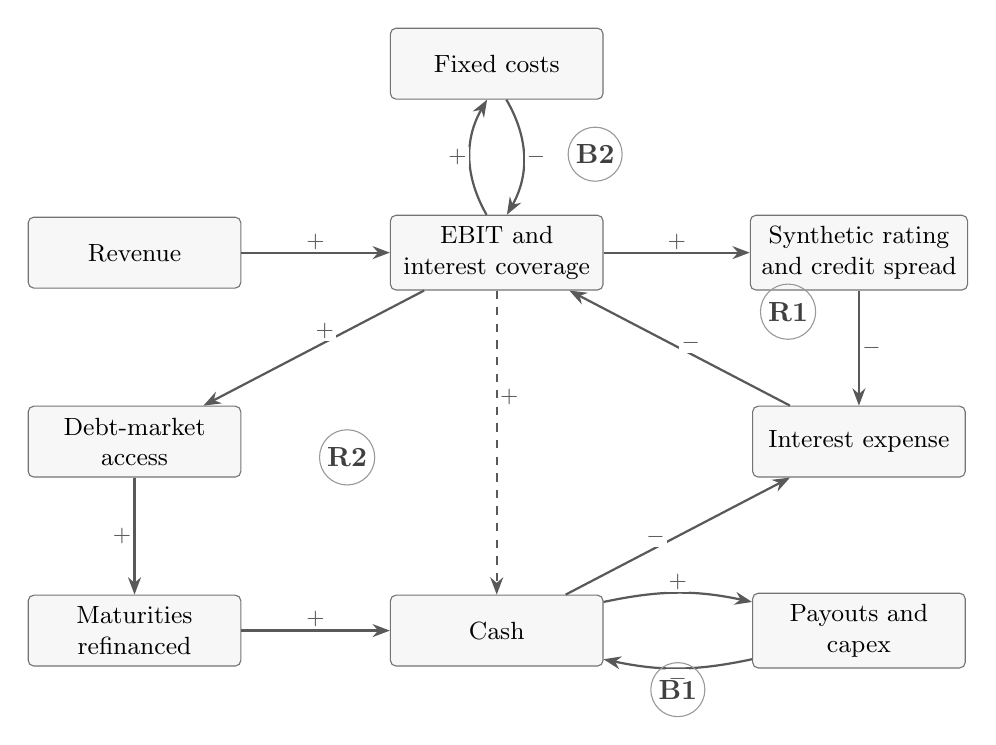
\begin{tikzpicture}[font=\small,
  var/.style={draw=black!55, rounded corners=2pt, fill=black!3, inner sep=4pt, align=center, minimum width=27mm, minimum height=9mm},
  arr/.style={-{Stealth[length=2.2mm]}, thick, black!65},
  lab/.style={font=\footnotesize, fill=white, inner sep=0.8pt},
  loop/.style={font=\bfseries, black!75, circle, draw=black!40, inner sep=1.5pt}]
\node[var] (fixed) at (0, 2.4) {Fixed costs};
\node[var] (rev) at (-4.6, 0) {Revenue};
\node[var] (ebit) at (0, 0) {EBIT and\\interest coverage};
\node[var] (rating) at (4.6, 0) {Synthetic rating\\and credit spread};
\node[var] (access) at (-4.6, -2.4) {Debt-market\\access};
\node[var] (interest) at (4.6, -2.4) {Interest expense};
\node[var] (refi) at (-4.6, -4.8) {Maturities\\refinanced};
\node[var] (cash) at (0, -4.8) {Cash};
\node[var] (payouts) at (4.6, -4.8) {Payouts and\\capex};
\draw[arr] (rev) -- node[lab, above]{$+$} (ebit);
\draw[arr] (ebit) -- node[lab, above]{$+$} (rating);
\draw[arr] (rating) -- node[lab, right]{$-$} (interest);
\draw[arr] (interest) -- node[lab, above, pos=0.45]{$-$} (ebit);
\draw[arr] (ebit) -- node[lab, above, pos=0.45]{$+$} (access);
\draw[arr] (access) -- node[lab, left]{$+$} (refi);
\draw[arr] (refi) -- node[lab, above]{$+$} (cash);
\draw[arr] (cash) -- node[lab, above, pos=0.4]{$-$} (interest);
\draw[arr] (cash.15) to[bend left=12] node[lab, above]{$+$} (payouts.165);
\draw[arr] (payouts.195) to[bend left=12] node[lab, below]{$-$} (cash.345);
\draw[arr] (ebit.105) to[bend left=30] node[lab, left]{$+$} (fixed.255);
\draw[arr] (fixed.285) to[bend left=30] node[lab, right]{$-$} (ebit.75);
\draw[arr, dashed] (ebit) -- node[lab, right, pos=0.35]{$+$} (cash);
\node[loop] at (3.7, -0.75) {R1};
\node[loop] at (-1.9, -2.6) {R2};
\node[loop] at (2.3, -5.55) {B1};
\node[loop] at (1.25, 1.25) {B2};
\end{tikzpicture}
\caption{The four feedback loops in causal-loop notation. A ``$+$'' (``$-$'') link means that the variables move in the same (opposite) direction; a loop is reinforcing (R) when the product of its signs is positive and balancing (B) when it is negative. R1, leverage--spread spiral; R2, market-access cliff; B1, cash conservation; B2, delayed restructuring. The dashed link (operating cash flow) is not part of a loop. The full model also contains working capital, customer deposits, the debt-maturity ladder, taxes and the recession regime.}
\label{fig:loops}
\end{figure}

\section{Evaluation design}\label{sec:design}

\subsection{Pre-specification and its history}\label{sec:prespec}
The decision rule for H2 was committed before the first full-sample run of the second version (commit \texttt{460cdda}) and is unchanged. The plan for this revision (\texttt{docs/REVISION\_PLAN\_3.md}, commit \texttt{70c4b17}) was committed before any revision-3 code change or run. It lists the corrections, the three specifications, the ladder, the tests of both pillars and their success criteria, and what the revision does not attempt. Two supplements followed, each before the results they govern: the first (commit \texttt{6d5ea9c}, the same day) fixed the definition of a realized shortfall, the merger exclusion and the walk-forward grids; the second (commit \texttt{6ca96b7}) was written after a timing probe of 60 firms that produced no test statistics. It added the confirmatory test of v3 against v2-pre, defined the ladder on a fixed sample of 1{,}000 firms, and kept the Monte Carlo design unchanged. A dry run of the whole pipeline on 300 firms and three cutoffs checked that every test ran; by the plan's rule its statistics changed no rule or constant and do not enter the paper.

Two choices were made after the plan and before any full-sample result, and we state them because the plan did not settle them. First, B2 has eight cells (two horizons, two scenario versions, two labels). The plan names one test; in implementing it we chose the eight-quarter Recession-scenario cell of the shortfall label, because it is the only cell with enough cutoff years for a year-block interval, while an internal planning note had named the realized-shock version. All cells give the same verdict (Table~\ref{tab:shortfall}). Second, a reviewer's comment led us to add, as exploratory analyses outside every confirmatory test, rivals that use no accounting data (firm age, restatements, late filings and the industry's base rate) and a robustness pass in which co-registrants that share filings count as one firm.

The full run took place on 13--14 November 2026 on x86 servers, every stage on the same architecture, with code digest, lock file and snapshot digest recorded beside each result. Earlier attempts at the full run were lost before their outputs were retrieved and produced no statistics.

\subsection{Pillar A: transmission}
For every firm and every cutoff (15 February 2014--2024), the simulator is calibrated on the filings available at the cutoff. We replace its simulated revenue with the revenue the company actually reported over the following eight quarters and run 500 paths; the point forecast is the median of the paths' cumulative operating cash flow (and of FCF). The outcome is cumulative operating cash flow over the eight quarters as a percentage of revenue in the four quarters before the cutoff. Every rival sees the same realized revenue, quarter by quarter:
\begin{enumerate}[label=N\arabic*]
\item the trailing four-quarter cash-flow margin times revenue;
\item the same over eight quarters;
\item the same over 16 quarters, the window of the simulator's cost regression;
\item the four-quarter margin shrunk toward the leave-one-out median margin of the firm's industry in the same year, with the weight chosen each year on earlier years;
\item a per-firm regression of quarterly cash flow on revenue over 16 quarters (a fixed and a variable part: operating leverage without simulation);
\item the same regression with the change in revenue added (working-capital timing).
\end{enumerate}
\noindent T0 is the simulator with its four feedback loops switched off and T1 the full simulator.

\paragraph{Confirmatory tests.} (i) \emph{v3 against v2-pre} (S1): the statistic is the difference between the median absolute errors of the two specifications on the firm-years that both forecast. The decision uses a $t(G-1)$ interval over the $G$ yearly differences of medians; the test succeeds if its upper 95\% bound is below zero. A year-block bootstrap and a Diebold--Mariano test of the mean difference with firm$\times$year clustering accompany it. (ii) \emph{H2}, by the rule of the second version: the incremental Spearman correlation of (T1 $-$ base) with (realized $-$ base) has a 95\% interval above zero against each of N3, N4 and N6, and T1's coefficient in an encompassing regression of the realized departure from N1 on the departures of T1, N3, N4 and N6 is significant at 5\%. (iii) \emph{Elasticity}: the ratio of the simulator's to the realized response of cash flow to revenue changes lies in $[0.8, 1.25]$. The plan states that beating the 16-quarter margin is not required and that a failure to do so is reported as it is.

\paragraph{Encompassing and combinations.} Encompassing regressions are reported with two-way clustered standard errors and $t(G-1)$ critical values, and under absolute loss: a pairwise absolute-loss encompassing test and a median (LAD) regression of the outcome on the forecasts in levels \citep{fair1990}. Combinations add a fraction $\lambda$ of one forecast's departure to a base, $\text{N3}+\lambda(\text{T1}-\text{N3})$, with $\lambda$ chosen each test year on earlier years and outcomes winsorized only at bounds from those years. Gains are tested with a Diebold--Mariano test under firm$\times$year clustering and a year-block bootstrap that re-estimates $\lambda$ in each resample, and reported year by year.

\paragraph{The family.} The pre-specified family has 16 comparisons: the simulator, the margin plus the simulator, the margin plus the four-quarter margin and the margin plus the regression, each against N3, for operating cash flow and FCF, under median and mean absolute error. We control its familywise error with the studentized stepwise method of \citet{romano2005} ($B=\FamB$, firm$\times$year bootstrap), and report Holm's adjustment for continuity with the second version. Over all forecasters we compute the model confidence set at $\alpha=0.10$ \citep{hansen2011} and Hansen's test for superior predictive ability against N3.

\subsection{Pillar B: distribution and stress}
\paragraph{B1, density.} The same runs give each firm-year a predictive distribution of eight-quarter cash flow given realized revenue. Its rivals are a Gaussian and an empirical distribution of the residuals of the 16-quarter margin, estimated on cutoffs up to $Y-3$. We compute the CRPS of each and the PIT histogram, and test the CRPS differences with a Diebold--Mariano test under firm$\times$year clustering. Success requires the simulator's CRPS to be lower than a rival's with $p<0.05$.

\paragraph{B2, liquidity shortfall.} The forecast is the share of paths on which cash plus undrawn committed credit falls below zero within $k\in\{4,8\}$ quarters, under the Recession preset or, for 2020 and 2022, under each firm's industry's realized revenue shock. A realized shortfall is a credit event (an 8-K Item 1.03, 2.04 or 3.01; an acceleration or delisting notice filed with a completed acquisition or change of control is excluded) or cash below 25\% of its opening level together with an increase in total debt above 5\% of trailing revenue. Rivals are a logit on opening cash to revenue, debt to assets and FCF margin, and Altman's Z$''$, both trained only on labels observable at the cutoff. Scores are the Brier and log scores with Murphy's decomposition and reliability curves. Success requires a Brier skill score above zero against the logit with a year-block interval that excludes zero. Firm-years inside a bankruptcy are excluded.

\paragraph{B3, credit events (secondary).} The AUC of the simulator's baseline health score and breach probabilities for a bankruptcy petition and for the broader credit-event label.

\subsection{Inference}
Common shocks within a year matter for every test, and there are at most eleven cutoffs. We therefore cluster by firm and year \citep{cameron2011}, use $t(G-1)$ critical values with $G$ the number of years, report whether two-way variance matrices are positive semi-definite, and use year-block bootstraps where the decision depends on few years. Out-of-sample logits are ridge-penalized and trained, for test year $Y$, on cutoffs up to $Y-3$. Only the tests named above are confirmatory; S1, B1 and B2 are single tests outside the family of 16. Monte Carlo seeds are common to all firms and specifications, so simulation noise is common across the comparisons.

\section{Pillar A: transmission}\label{sec:pillarA}

\subsection{The corrected specification against the old one}
Table~\ref{tab:specs} reports the headline numbers of every specification on the same \SpecN{} firm-years. The pre-specified confirmatory test compares v3 with v2-pre on the \SOneN{} firm-years that both forecast. The median absolute error falls from \SOneMedVtwo{} to \SOneMedVthree{} percentage points of revenue (difference \SOneStat); the $t(\SOneG-1)$ interval of the yearly differences is \SOneLo{} to \SOneHi{}, the year-block interval \SOneBlockLo{} to \SOneBlockHi{}, and the difference is negative in all \SOneNeg{} years. The test \SOneVerdict. The improvement is in the typical error, not the mean: the mean absolute difference is positive, \SOneDmMean{} points in v3's disfavour, though not significantly (Diebold--Mariano $p=\SOneDmP$). The corrected model has heavier tails, a point we return to in pillar B.

\begin{table}[t]
\centering\scriptsize
\caption{The three specifications on the same firm-years}
\label{tab:specs}
\begin{tabular}{lrrrrrrr}
\toprule
 & \multicolumn{2}{c}{Median abs.\ error} & Elasticity & Incr.\ $\rho$ & Enc.\ $t$ & Bankr. & Mean CRPS \\
\cmidrule(lr){2-3}
Specification & Simulator & 16q margin & ratio & vs 16q & (firm$\times$year) & AUC & (simulator) \\
\midrule
v2-pre (prior 35\%) & 11.1 & 6.7 & 2.18 & 0.22 & 8.7 & 0.87 & 26 \\
v2-rev (prior 5\%) & 8.8 & 6.7 & 1.24 & 0.23 & 8.7 & 0.87 & 24 \\
v3, default $\tau$, $\lambda$ & 8.1 & 6.7 & 0.88 & 0.24 & 10.3 & 0.87 & 132 \\
v3, walk-forward $\tau$, $\lambda$ & 8.1 & 6.7 & 0.67 & 0.23 & 8.4 & 0.87 & 207 \\
\bottomrule
\end{tabular}

\par\smallskip
\begin{minipage}{\linewidth}\footnotesize
Errors: median absolute error of eight-quarter operating cash flow, percentage points of trailing revenue. Elasticity ratio: the model's over the realized slope of cash flow on the revenue change (pre-specified range 0.8--1.25). Incr.\ $\rho$: incremental Spearman correlation against the 16-quarter margin. Enc.\ $t$: the simulator's $t$-statistic in the encompassing regression, two-way clustered. Bankruptcy AUC: baseline health score, petition within eight quarters. Mean CRPS: B1, operating cash flow.
\end{minipage}
\end{table}

Where does the improvement come from? The ladder in Table~\ref{tab:ladder} adds the corrections one at a time on a fixed sample of \LadN{} firms. It is descriptive, by the plan. The consistent residual and tax (F5) lowers the median error from \LadPre{} to \LadFive; the posterior cost prior (F1) brings it to \LadOne; the rest of v3 to \LadThree. Most of the gain comes from the cost prior: v2-pre shrank every firm's costs toward a 35\% fixed share with roughly two-thirds of the weight on the prior however much its revenue had varied. The corrections to the data layer change the sample more than the errors (the legacy layer gives \LadLegacy{} on \LadLegacyN{} firm-years).

\begin{table}[t]
\centering\scriptsize
\caption{The ladder of corrections (descriptive; fixed sample of 1{,}000 firms)}
\label{tab:ladder}
\begin{tabular}{lrrrr}
\toprule
Rung & Firm-years & Simulator median abs.\ error & 16q margin & Elasticity ratio \\
\midrule
v2-pre, legacy data layer & 3{,}216 & 11.72 & 7.09 & 2.98 \\
v2-pre & 2{,}981 & 11.45 & 6.81 & 2.45 \\
+ F5 (consistent CFO residual and tax) & 2{,}981 & 10.48 & 6.81 & 2.71 \\
+ F4 (missing D\&A) & 2{,}981 & 10.41 & 6.81 & 2.69 \\
+ F1 (posterior cost prior, default $\tau$) & 2{,}981 & 8.91 & 6.81 & 1.89 \\
+ F2 (annual operating leverage) & 2{,}981 & 8.85 & 6.81 & 1.68 \\
+ F3 and the rest = v3 (defaults) & 2{,}981 & 8.33 & 6.81 & 0.82 \\
v3, walk-forward $\tau$ and $\lambda$ & 2{,}981 & 8.39 & 6.81 & 0.81 \\
\bottomrule
\end{tabular}

\par\smallskip
\begin{minipage}{\linewidth}\footnotesize
Corrections added cumulatively in the pre-specified order. The legacy data layer row uses the second version's loader, so its firm-years differ.
\end{minipage}
\end{table}

\subsection{Levels and the response to revenue}
The correction does not change the ranking of the models in levels (Table~\ref{tab:transmission}, Figure~\ref{fig:ladder}). The 16-quarter margin is the most accurate model, with a median absolute error of \TrMaeNthree{} percentage points; the four-quarter margin reaches \TrMaeNone, the regressions \TrMaeNfive{} and \TrMaeNsix, and the simulator \TrMaeTone{} (\TrMaeTzero{} without loops). In the family, the simulator alone is worse than the margin by \FamTwinMedDiff{} points of median error (Romano--Wolf $p=\FamTwinMedRw$).

The direction of its errors has changed. In a regression of each eight-quarter total on the revenue change, v2-pre's cash flow responded \ElastVtwopre{} times as strongly as firms' does: its fixed-cost prior turned revenue changes into cash changes that were too large. Under v3 the ratio is \ElastRatioExact{} (simulator \ElastCfoTwin, realized \ElastCfoReal), \ElastVerdict{} the pre-specified range of 0.8--1.25, so the elasticity criterion fails. With the default hyper-parameters the ratio is \ElastVthreedef, inside the range. The walk-forward rule chose weak cost priors ($\tau=\SelTauMode$ in most years, no prior in the first) and fixed costs that adjust to permanent revenue changes at $\lambda=\SelLamMin$--\SelLamMax. These choices lower the median error slightly, but together they make costs too variable: the model now underreacts. The selection criterion was the median error, not the elasticity, and we report the conflict rather than resolve it.

\begin{figure}[t]
\centering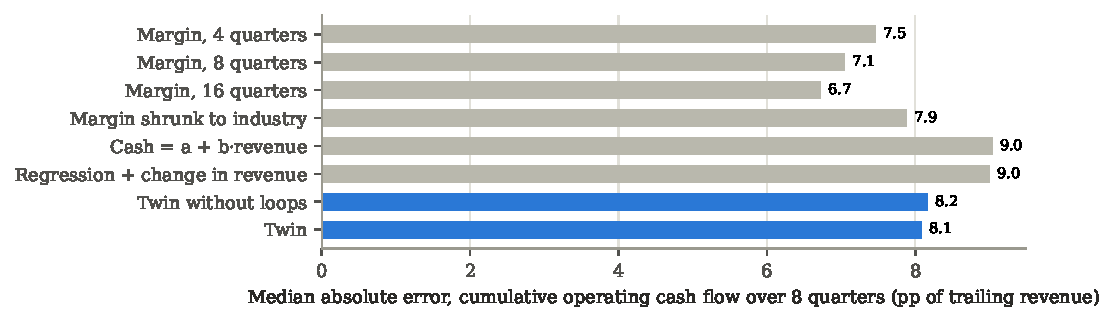
\includegraphics[width=\linewidth]{figures/ladder.pdf}
\caption{Median absolute error of eight models of cumulative operating cash flow over the eight quarters after each cutoff, given the realized revenue path (v3); \TrN{} firm-years, 2014--2024.}
\label{fig:ladder}
\end{figure}

\begin{table}[t]
\centering\scriptsize
\caption{Transmission: realized revenue given to the simulator and to six simple rules (v3)}
\label{tab:transmission}
\resizebox{\linewidth}{!}{%
\begin{tabular}{lrrrllrr}
\toprule
 & \multicolumn{5}{c}{Operating cash flow} & \multicolumn{2}{c}{Free cash flow} \\
\cmidrule(lr){2-6}\cmidrule(lr){7-8}
 & \multicolumn{2}{c}{Error (pp of revenue)} & & \multicolumn{2}{c}{Incremental $\rho$ against} & Median & Incr.\ $\rho$ \\
\cmidrule(lr){2-3}\cmidrule(lr){5-6}
Model & Median & Mean & $\rho$ & 4-quarter margin [95\% CI] & 16-quarter margin [95\% CI] & error & vs.\ 16q \\
\midrule
Margin, 4 quarters & 7.5 & 13.0 & 0.77 &   & 0.21  & 8.1 & 0.19 \\
Margin, 8 quarters & 7.1 & 12.5 & 0.78 & 0.31 [0.29, 0.33] & 0.13  & 7.6 & 0.10 \\
Margin, 16 quarters & 6.7 & 12.1 & 0.80 & 0.40 [0.38, 0.42] &   & 7.0 &  \\
Margin shrunk to industry & 7.9 & 13.2 & 0.76 & 0.14 [0.12, 0.15] & 0.20  & 8.2 & 0.21 \\
\addlinespace
Cash = $a + b\cdot$revenue & 9.0 & 14.8 & 0.75 & 0.26 [0.24, 0.28] & 0.18  & 9.8 & 0.17 \\
Regression + change in revenue & 9.0 & 15.2 & 0.74 & 0.25 [0.23, 0.27] & 0.19  & 9.8 & 0.18 \\
\addlinespace
Twin without loops & 8.2 & 14.5 & 0.75 & 0.37  & 0.23  & 8.8 & 0.22 \\
Twin & 8.1 & 14.2 & 0.76 & 0.38 [0.36, 0.40] & 0.23 [0.21, 0.25] & 8.7 & 0.23 \\
\bottomrule
\end{tabular}}

\par\smallskip
\begin{minipage}{\linewidth}\footnotesize
Outcome: cumulative operating (free) cash flow over the eight quarters after the cutoff, percentage points of trailing revenue. Errors: median and winsorized mean absolute error. $\rho$: Spearman correlation with the realized outcome. Incremental $\rho$: correlation of (model $-$ base) with (realized $-$ base); firm-clustered bootstrap CI.
\end{minipage}
\end{table}

The test needs eight reported quarters after the cutoff, so it conditions on survival. \AttrShare{} of the firm-years qualify, but only \AttrShareBk{} of those followed by a bankruptcy petition, against \AttrShareNonBk{} of the others. Reweighting by the inverse of the estimated probability of survival changes the median errors little (simulator \AttrTwinIpw, 16-quarter margin \AttrSixteenIpw): the ranking of the models does not depend on the selection, but the transmission results say little about firms in their last quarters before failure.

\subsection{Information beyond the rules}
Against the four-quarter margin the simulator's incremental correlation is \TrIncrTwin{} (95\% CI \TrIncrTwinLo--\TrIncrTwinHi), and the 16-quarter margin's is \TrIncrSixteen{}: against a noisy base, any less noisy estimate of the persistent margin looks informative. Against the stronger bases the simulator still carries information: its incremental correlation with the residual of the 16-quarter margin is \TrTwinVsSixteen{} (CI \TrTwinVsSixteenLo--\TrTwinVsSixteenHi), of the shrunk margin \TrTwinVsShrunk{} and of the regression with timing \TrTwinVsReg. In the encompassing regression (Appendix Table~\ref{tab:encompassing}) its $t$-statistic is \TrEncTwinT{} with firm clustering and \TrEncTwinTTwoWay{} with firm and year clustering. By the pre-specified rule, H2 \TrVerdict, as it did in every specification (Table~\ref{tab:specs}).

The rule was written for squared loss, and the encompassing evidence depends on it. With $t(G-1)$ critical values the two-way $t$-statistic is \EncTGOne{} against a critical value of \EncTGOneCrit{}, but the two-way variance matrix of that regression is \EncTGOnePsd, so this number should be read with care. Under absolute loss the evidence disappears. The pairwise test that the 16-quarter margin encompasses the simulator gives $t=\EncAbsSixteen$ (one-sided $p=\EncAbsSixteenP$), and in a median regression of the outcome on all five forecasts the simulator's coefficient is \EncLadCoef{} ($t=\EncLadT$), while the timing regression keeps a significant weight ($t=\EncLadRegT$). The simulator's departures from persistence are informative about the mean of cash flow, which large errors dominate, not about the typical firm.

\subsection{How much it is worth}
Table~\ref{tab:family} and the combinations measure that information out of sample. Adding a fraction $\lambda$ of the simulator's departure to the 16-quarter margin, with $\lambda$ between \LamMin{} and \LamMax{} in every year, lowers the mean absolute error by \GainPct{} (year-block CI \GainLo--\GainHi), in \GainPos{} of \GainYears{} years (Diebold--Mariano $p=\GainDmP$); for FCF the gain is \GainFcfPct. Combining forecasts helps even when the second forecast is worse \citep{bates1969,clemen1989,timmermann2006}, so the relevant comparison is with the margin combined in the same way with a simple rule. Against the margin combined with the cash-revenue regression, the simulator's combination is better by \GainRegPct{} of the error (CI \GainRegLo--\GainRegHi); against the margin combined with the four-quarter margin, by \GainFourPct{} with an interval that includes zero (\GainFourLo--\GainFourHi; positive in \GainFourPos{} of \GainYears{} years). The loops contribute almost nothing: the combination built from the loop-free simulator is only \GainLoopsPct{} worse.

In the family of 16, \FamRejects{} comparisons reject at 5\% after the Romano--Wolf correction. The simulator alone is worse than the margin in all four cells. The margin plus the simulator is better than the margin under mean absolute error (by \FamCombMeanDiff{} points, $p=\FamCombMeanRw$) but not under median absolute error (\FamCombMedDiff, $p=\FamCombMedRw$); the margin plus the regression is also better under mean error ($p=\FamRegMeanRw$). Hansen's test rejects that no member of the family beats the margin under mean error ($p=\SpaCfoMean$ for operating cash flow, \SpaFcfMean{} for FCF) but not under median error ($p=\SpaCfoMed$ and \SpaFcfMed). The model confidence set for the median error of operating cash flow contains \McsSize{} of the 19 forecasters: it excludes the simulator alone ($p_{\mathrm{MCS}}=\McsTwinP$) and contains the 16-quarter margin and every combination built on it. The simulator's combination is the last model standing ($p_{\mathrm{MCS}}=\McsCombP$), but at this level the data cannot distinguish it from the margin alone or from the margin's other combinations.

\begin{table}[t]
\centering\scriptsize
\caption{The pre-specified family of 16 comparisons against the 16-quarter margin}
\label{tab:family}
\begin{tabular}{llrrrrr}
\toprule
Outcome, loss & Forecast & $\Delta$ vs 16q & 95\% CI & $p$ & Romano--Wolf & Holm \\
\midrule
CFO, median & Twin & 1.27 & [0.83, 1.92] & $<$0.001 & 0.004 & 0.011 \\
CFO, median & 16q + twin & $-$0.20 & [$-$0.36, 0.05] & 0.081 & 0.370 & 0.651 \\
CFO, median & 16q + 4q & 0.05 & [$-$0.35, 0.52] & 0.823 & 0.992 & 1.000 \\
CFO, median & 16q + regression & 0.01 & [$-$0.15, 0.20] & 0.942 & 0.993 & 1.000 \\
CFO, mean & Twin & 1.79 & [1.15, 2.49] & $<$0.001 & 0.001 & 0.002 \\
CFO, mean & 16q + twin & $-$0.38 & [$-$0.58, $-$0.16] & 0.005 & 0.021 & 0.048 \\
CFO, mean & 16q + 4q & $-$0.11 & [$-$0.60, 0.44] & 0.650 & 0.975 & 1.000 \\
CFO, mean & 16q + regression & $-$0.24 & [$-$0.39, $-$0.12] & 0.002 & 0.020 & 0.021 \\
FCF, median & Twin & 1.28 & [0.64, 2.11] & 0.004 & 0.025 & 0.048 \\
FCF, median & 16q + twin & $-$0.15 & [$-$0.42, 0.10] & 0.254 & 0.738 & 1.000 \\
FCF, median & 16q + 4q & 0.02 & [$-$0.31, 0.40] & 0.927 & 0.993 & 1.000 \\
FCF, median & 16q + regression & $-$0.05 & [$-$0.24, 0.14] & 0.620 & 0.975 & 1.000 \\
FCF, mean & Twin & 1.79 & [1.10, 2.53] & $<$0.001 & 0.002 & 0.002 \\
FCF, mean & 16q + twin & $-$0.44 & [$-$0.67, $-$0.17] & 0.005 & 0.025 & 0.048 \\
FCF, mean & 16q + 4q & $-$0.21 & [$-$0.64, 0.28] & 0.337 & 0.816 & 1.000 \\
FCF, mean & 16q + regression & $-$0.25 & [$-$0.41, $-$0.11] & 0.003 & 0.027 & 0.041 \\
\bottomrule
\end{tabular}

\par\smallskip
\begin{minipage}{\linewidth}\footnotesize
$\Delta$: difference in median or mean absolute error (percentage points of revenue), positive when the forecast is worse than the margin. Combinations use year-by-year $\lambda$ chosen on earlier years. CI and $p$: firm$\times$year bootstrap; Romano--Wolf: studentized stepwise familywise $p$-value; Holm: for continuity with the second version.
\end{minipage}
\end{table}

\section{Pillar B: distribution and stress}\label{sec:pillarB}

\subsection{Density of cash flow given revenue}
Table~\ref{tab:density} reports B1 on \DenN{} firm-years. The simulator fails against both rivals. Its mean CRPS for operating cash flow is \DenCrpsTwin, against \DenCrpsGauss{} for the Gaussian and \DenCrpsEmp{} for the empirical residual distribution; neither difference is significant, because the CRPS differences are extremely heavy-tailed and a single year (\DenWorstYear, mean difference \DenWorstDiff) dominates them. By year, the simulator has the lower mean CRPS than the Gaussian in \DenBetterGauss{} of \DenYears{} years but than the empirical distribution in only \DenBetterEmp.

The PIT histogram shows why. \DenPitTails{} of outcomes fall in the outer deciles of the simulator's distribution (\DenPitLow{} in the lowest, \DenPitHigh{} in the highest), against 20\% for a calibrated forecast and \DenPitEmpTails{} for the empirical rival, and its 90\% interval covers \DenCov{} of outcomes (\DenCovFcf{} for FCF). Given the realized revenue, the only uncertainty left in the model is in costs, working capital and financing, and its shock processes put far too little of it there. The corrections made this worse in the mean: the corrected shock process has heavier tails, and the mean CRPS rises from \CrpsVtwopre{} under v2-pre to \CrpsVthree{} under v3 (Table~\ref{tab:specs}). The distributions that the simulator reports are statements about simulated paths, not calibrated forecasts. Online conformal rescaling of the quarterly intervals, reported in the appendix, restores average coverage of four-quarter forecasts but not in the stress year.

\begin{table}[t]
\centering\scriptsize
\caption{B1: predictive distributions of eight-quarter cash flow given realized revenue}
\label{tab:density}
\begin{tabular}{llrrrrrr}
\toprule
Outcome & Benchmark & Mean CRPS & Mean CRPS & DM $t$ & $p$ & Years sim. & Verdict \\
 & & (simulator) & (benchmark) & (firm$\times$year) & & better & \\
\midrule
CFO & Gaussian & 206.8 & 109.9 & 0.55 & 0.597 & 6/8 & failure \\
CFO & Empirical & 206.8 & 29.1 & 1.02 & 0.342 & 2/8 & failure \\
FCF & Gaussian & 219.9 & 93.3 & 0.67 & 0.522 & 6/8 & failure \\
FCF & Empirical & 219.9 & 26.7 & 1.03 & 0.339 & 3/8 & failure \\
\bottomrule
\end{tabular}

\par\smallskip
\begin{minipage}{\linewidth}\footnotesize
CRPS in percentage points of trailing revenue. Rivals: Gaussian and empirical distributions of the residuals of the 16-quarter margin, estimated on cutoffs up to $Y-3$. DM $t$: Diebold--Mariano statistic of the CRPS difference (positive: simulator worse), clustered by firm and year. Years twin better: test years in which the simulator's mean CRPS is lower. Verdict: the pre-specified rule ($p<0.05$ in the simulator's favour).
\end{minipage}
\end{table}

\subsection{Liquidity shortfall}
Table~\ref{tab:shortfall} reports B2. In the primary cell (eight quarters, Recession preset; \ShortN{} firm-years, \ShortEv{} shortfalls), the simulator's Brier score is \ShortBrierTwin{} against \ShortBrierLogit{} for the logit, a Brier skill score of \ShortBss{} with a year-block interval of \ShortBssLo{} to \ShortBssHi. The test \ShortVerdict. Every other cell, including the version that gives each firm its industry's realized revenue shock, gives a negative skill score as well.

The decomposition locates the failure. The simulator's reliability term (\ShortRel) is far larger than its resolution (\ShortRes): its probabilities are badly calibrated, and they separate firms only a little. Its average probability is \ShortMeanP{} against a realized rate of \ShortBase{}; \ShortLowBinShare{} of firm-years receive a probability below 10\%, and \ShortLowBinRate{} of those suffer a shortfall. Most shortfalls happen to firms whose simulated paths never run out of liquidity. Two reasons are plausible: the model's treasury refinances maturities and draws credit lines that, in reality, the firm did not or could not use, and the label also counts credit events, such as delisting notices, that do not follow from a lack of cash.

\begin{table}[t]
\centering\scriptsize
\caption{B2: probability of a liquidity shortfall}
\label{tab:shortfall}
\begin{tabular}{lllrrrrrrrr}
\toprule
Label & Horizon & Scenario & Firm-years & Events & \multicolumn{3}{c}{Brier score} & BSS vs & Log score & Sim. \\
\cmidrule(lr){6-8}
 & & & & & Sim. & Logit & Z$''$ & logit & sim./logit & rel./res. \\
\midrule
Shortfall & 4q & industry shock & 2{,}322 & 181 & 0.080 & 0.071 & 0.071 & $-$0.12 & 0.67/0.27 & 0.009/0.001 \\
Shortfall & 4q & Recession & 9{,}944 & 809 & 0.085 & 0.074 & 0.073 & $-$0.15 & 0.66/0.28 & 0.011/0.001 \\
Shortfall & 8q & industry shock & 2{,}286 & 334 & 0.149 & 0.123 & 0.123 & $-$0.22 & 1.18/0.41 & 0.026/0.001 \\
Shortfall & 8q & Recession & 8{,}818 & 1{,}344 & 0.152 & 0.127 & 0.126 & $-$0.20 & 1.13/0.42 & 0.026/0.003 \\
Credit event & 4q & industry shock & 2{,}738 & 105 & 0.041 & 0.037 & 0.037 & $-$0.12 & 0.33/0.16 & 0.005/0.000 \\
Credit event & 4q & Recession & 13{,}119 & 528 & 0.047 & 0.038 & 0.038 & $-$0.22 & 0.34/0.17 & 0.009/0.000 \\
Credit event & 8q & industry shock & 2{,}738 & 194 & 0.078 & 0.065 & 0.065 & $-$0.19 & 0.57/0.25 & 0.013/0.001 \\
Credit event & 8q & Recession & 13{,}119 & 982 & 0.083 & 0.069 & 0.068 & $-$0.21 & 0.57/0.26 & 0.016/0.002 \\
\bottomrule
\end{tabular}

\par\smallskip
\begin{minipage}{\linewidth}\footnotesize
Forecast: share of paths with cash plus undrawn committed credit below zero within the horizon. Realized: credit event (8-K Item 1.03, 2.04, 3.01) or cash below 25\% of opening with debt up by more than 5\% of trailing revenue. Industry's realized shock: cutoffs 2020 and 2022 only. Logit: opening cash/revenue, debt/assets and FCF margin; logit and Altman Z$''$ trained on labels observable at the cutoff. BSS: Brier skill score $1-\mathrm{BS}_{\text{twin}}/\mathrm{BS}_{\text{logit}}$. Rel./res.: the simulator's reliability and resolution \citep{murphy1973}. The primary cell is eight quarters under the Recession preset.
\end{minipage}
\end{table}

\subsection{Credit events}
As a ranking device the simulator does better (Table~\ref{tab:credit}). Its baseline health score predicts a bankruptcy petition within eight quarters with an AUC of \BkAucTwin, against \BkAucZ{} for Altman's Z$''$, and the broader credit event (\CeEv{} events) with \CeAucTwin{} against \CeAucZ. Its breach probabilities, the quantity B2 scores, rank firms less well than its health score. A score that ranks well but whose probabilities are miscalibrated can be recalibrated; but the health score ranks no better than its own formula applied to the opening balance sheet without simulation (Section~\ref{sec:secondary}).

\begin{table}[t]
\centering\scriptsize
\setlength{\tabcolsep}{3pt}
\caption{B3: credit events within the horizon (AUC, 95\% CI)}
\label{tab:credit}
\resizebox{\linewidth}{!}{\begin{tabular}{lrrrrrr}
\toprule
Event & Firm-years & Events & Simulator health [95\% CI] & Breach prob. & Recession breach prob. & Altman Z$''$ \\
\midrule
Bankruptcy petition (1.03), 8q & 21{,}075 & 419 & 0.87 [0.85, 0.89] & 0.84 & 0.83 & 0.82 \\
Credit event (1.03, 2.04, 3.01), 8q & 19{,}266 & 1{,}539 & 0.66 [0.64, 0.68] & 0.63 & 0.63 & 0.64 \\
Credit event, 4q & 19{,}266 & 842 & 0.68 [0.66, 0.70] & 0.65 & 0.65 & 0.66 \\
Acceleration (2.04), 8q & 20{,}681 & 646 & 0.76 [0.74, 0.79] & 0.72 & 0.71 & 0.74 \\
Delisting notice (3.01), 8q & 19{,}657 & 1{,}295 & 0.66 [0.64, 0.68] & 0.64 & 0.64 & 0.64 \\
\bottomrule
\end{tabular}
}
\par\smallskip
\begin{minipage}{\linewidth}\footnotesize
Twin health: baseline health score (sign reversed). Breach probabilities: baseline and Recession preset, eight quarters. Credit event: 8-K Items 1.03, 2.04 or 3.01, excluding those filed with a completed acquisition or change of control.
\end{minipage}
\end{table}

\section{Secondary evidence}\label{sec:secondary}

\paragraph{Ranking firms (H1, descriptive).} On the census, across \BkPanN{} firm-years with \BkPanEv{} petitions within eight quarters at \BkPanFirms{} companies, the simulator's baseline score has an AUC of \BkPanTwin, its own scoring formula applied to the opening balance sheet without simulation \BkPanFormula{} (difference \BkPanFormulaDiff, $p\BkPanFormulaP$), Ohlson's O-score \BkPanOhlson{} and Altman's Z$''$ \BkPanAltman{} (Appendix Table~\ref{tab:bankruptcy}). Among the \BkWeakN{} firm-years that were already weak, which account for \BkWeakShare{} of petitions, the simulator reaches \BkWeakTwin{} and the formula \BkWeakFormula{} ($p\BkWeakFormulaP$ unadjusted; Holm-adjusted in Appendix Table~\ref{tab:holm}). For severe cash burn the simulator reaches \PanTwinAuc, below the trailing FCF margin (\PanFcfAuc), and for abnormal burn it has no skill (\PanAbnTwinAuc). H1, that the stress score ranks distress better than the trailing FCF margin and its own formula, is rejected.

\paragraph{Feedback loops (H3, descriptive).} Given realized revenue, the simulator's event probabilities add to a logit of a static runway rule and the scores \DecCashDelta{} in AUC for cash falling below half, \DecDebtDelta{} for new borrowing and \DecCapexDelta{} for capex cuts, with intervals above zero, and \DecDivDelta{} for dividend cuts, with an interval that touches zero (Appendix Table~\ref{tab:decisions}). Two loops are the only channel through which the model produces some events at all: without the market-access cliff its cash practically never falls below half (AUC \DecCashNoRtwo{} against \DecCashTwin), and without cash conservation dividends are never cut. By the rule written for it, H3 is \HThreeVerdict{}, but for those events the comparator never produces the event, so the gain is mechanical; at a 70\% cash threshold, where the loop-free model does produce it, it predicts slightly better (Appendix Table~\ref{tab:thresholds}). We read H3 as a statement about the model's structure.

\paragraph{Downturns as decompositions.} Given each industry's realized revenue shock in the 2015, 2020 and 2022 downturns, the simulator's fragility score is associated with abnormal cash burn in rank regressions that control for the shock, the FCF margin and the health formula ($t=\EpiFifteenTRobust$, \EpiTwentyTRobust{} and \EpiTwentyTwoTRobust{} with industry clustering; the pre-specified rule of the second version \EpiVerdict). Because the shock is realized, this is a decomposition, not a forecast: once the hit is known, the simulated fragility is associated with who bleeds most; filings cannot say whom a downturn will hit (online appendix).

\paragraph{Non-accounting rivals (exploratory).} Firm age, recent restatements and non-reliance filings, late-filing notices and the industry's base rate predict a petition with an AUC of \RivAucNonacc{} on \RivN{} test firm-years (\RivEv{} events), against \RivAucBench{} for the accounting benchmarks and \RivAucTwin{} for the simulator. Adding the simulator to both raises the AUC by \RivTwinBeyond{} (CI \RivTwinBeyondLo--\RivTwinBeyondHi). These rivals were added after the pre-specification and are exploratory.

\section{Discussion}\label{sec:discussion}

\paragraph{The verdicts.} Of the pre-specified tests, S1 succeeds, H2 survives by its rule, and the elasticity criterion, B1 and B2 fail. The corrections were real bug fixes and they improved the typical error, but they did not make the simulator better than persistence, they overshot the response to revenue, and they made the predictive distributions worse in the mean. A forecast user should read the results as follows.

\paragraph{Point forecasts.} The simulator's departures from a long-window margin carry information about mean cash flow, which a small weight on them recovers out of sample. The gain is a few percent of the mean absolute error, part of it is the generic gain from combining forecasts, it is absent under median loss, and the model confidence set does not separate it from the margin's other combinations. In practice a cash forecast should start from the long-window margin and move about a fifth of the way toward the simulation; the loops do not matter for this.

\paragraph{Uncertainty.} The simulator's distributions are too narrow and its shortfall probabilities miscalibrated, and neither failure is an accident of the shock process alone. Given the revenue path, the residual uncertainty in eight-quarter cash flow is dominated by things the model represents only as small mean-reverting shocks (accruals, one-off items, acquisitions and disposals), and the treasury rules let it finance what real firms did not. A simulator of this kind can give scenario arithmetic (how much new borrowing a stated revenue path requires, when maturities bind), but its path distribution should not be reported as a probability without recalibration against outcomes.

\paragraph{External validity.} The universe is US non-financial SEC filers with at least \$50 million of revenue. The pipeline depends on standardized, tagged, point-in-time disclosure, which exists in comparable form only under SEC XBRL and, since 2020--21, the European Single Electronic Format for annual reports. Among the \SmallN{} firm-years of firms with \$10--50 million of revenue, the pattern is the same: the simulator's median cash-flow error is \SmallMaeTwin{} against \SmallMaeSixteen{} for the 16-quarter margin, and its bankruptcy AUC \SmallAucTwin{} against \SmallAucFormula{} for its formula (\SmallBk{} petitions). Banks and insurers need a different balance-sheet model.

\paragraph{Limitations.} The transmission test uses realized revenue, so it cannot separate errors in the model's mechanics from noise in reported cash flow, and it conditions on eight quarters of survival. Bankruptcy and credit events are observed only through 8-K filings; firms that stop filing before petitioning, distressed exchanges and going-concern opinions are not counted. Industry codes are current, not point-in-time, and realized outcomes include later restatements. \AudGapsNew{} gaps remain in the quarterly panels. The model does not represent net operating losses or the interest-deduction limit, pensions, leases or captive finance operations, which matter for firms such as car makers; it uses no market inputs (returns, volatility, factor loadings), which a reviewer suggested and which structural credit models use; and its scenarios are named presets with sources rather than supervisory scenarios. Its structure and priors were designed in 2026 with knowledge of the 2014--2024 data, which no backtest can undo; the weekly rebuild of the public model now accumulates genuinely prospective forecasts.

\section{Conclusion}\label{sec:conclusion}
We built a transparent, automatically calibrated simulation model of the firm, corrected its implementation under rules written before any corrected result existed, and asked what it forecasts that persistence does not. The corrected model has a smaller typical error than the old one but is still less accurate than a 16-quarter cash-flow margin. What it adds to that margin is a small improvement in mean absolute error, which comes from its departures in large cases and is partly the generic benefit of combining forecasts. Its predictive distributions and shortfall probabilities are worse than simple statistical rivals. Filing-based simulation is useful as scenario arithmetic around a persistence forecast, not as a source of calibrated uncertainty. The design --- three specifications on a frozen snapshot, a ladder of simple rivals, encompassing under two losses, a controlled family of comparisons, and density and event scores against statistical rivals --- can be applied to any simulation model of the firm, and the data, code and tests are public so that others can be held to it.

\section*{Data and code availability}
All code, the point-in-time pipeline, the EDGAR universe and bankruptcy census, the frozen snapshot (digest \texttt{\SnapDigest}), the research experiments and the scripts that generate every table, figure and number in this paper are at \url{https://github.com/SpiliosDimakopoulos/fintwin} under the MIT license and archived on Zenodo (\href{https://doi.org/10.5281/zenodo.23434606}{doi:10.5281/zenodo.23434606}). The pre-specification is \texttt{docs/REVISION\_PLAN\_3.md}; its history is in the repository. An interactive version of the model is at \url{https://spiliosdimakopoulos.github.io/fintwin/}. All inputs are public: SEC EDGAR, FRED and the Philadelphia Fed Real-Time Data Set.

\section*{Use of AI tools}
Software development, data analysis and drafting were assisted by an AI coding assistant (Claude, Anthropic). The author designed the study, reviewed all code, results and text, and takes full responsibility for the content.

\section*{Acknowledgements}
I thank the researchers who commented on earlier versions; the null tests, the census of bankruptcies, the survivorship-free sample, the density and shortfall tests and the non-accounting rivals respond to their comments.

\bibliographystyle{elsarticle-harv}
\bibliography{references}

\appendix
\section{Additional tables}\label{app:tables}
Unless a caption says otherwise, every table in the appendices uses v3 with its walk-forward hyper-parameters, the full run on the frozen snapshot and the EDGAR universe (cutoffs 2014--2024, eight-quarter horizon). The online supplementary material also reports results from the earlier evaluation's design: the four-quarter forecasts use S\&P~500 members (today's, a sample selected on survival, and those of 2020), and the 2020 analyses use firms alive on 20 February 2020. Their samples, and therefore some AUCs and counts, differ from those of the main text.

\begin{table}[!htbp]
\centering\scriptsize
\caption{Calibrated parameters}
\label{tab:params}
\begin{tabular}{lp{0.5\linewidth}l}
\toprule
Parameter & Estimate & Window \\
\midrule
Seasonal factors $S_q$ & median ratio to centred 4-quarter moving average & last 32 quarters \\
Trend growth $\mu$ & median log growth, shrunk 50\% toward 1.2\%/quarter & last 12 quarters \\
AR coefficient $\phi$, volatility $\sigma_g$ & OLS; median absolute deviation of residuals & last 32 quarters \\
Tail index & Student-$t$ maximum likelihood on standardized residuals & growth residuals \\
Cyclicality $\beta$ & regression of revenue on real-time nominal GDP growth, shrunk 50\% toward 1.5 & last 40 quarters \\
Recession entry and exit & NBER recessions since 1947 & FRED \\
Fixed costs $F$, variable ratio $v$ & v3: posterior of a regression of cash costs on revenue (four-quarter changes), prior s.d.\ $\tau$ walk-forward; v2: penalized regression, prior 35\% (v2-pre) or 5\% (v2-rev) fixed & last 16 quarters \\
Fixed-cost adjustment $\lambda$ & v3: partial adjustment to permanent revenue changes, walk-forward & --- \\
Margin shock $m_t$ & AR(1) of cost-regression residuals; correlation with demand & last 16 quarters \\
DSO, DIO, DPO, deposit days & averages of balance to revenue or costs & last 4 quarters \\
Depreciation, capex, SBC ratios & medians & last 8 quarters \\
Coupon & interest expense over debt & last 4 quarters \\
Rollover share & two-year debt trend relative to maturities & last 8 quarters \\
Discretionary financing volatility & robust s.d.\ of quarterly debt changes & last 20 quarters \\
Maturity ladder & XBRL maturity schedule, else six-year average life & latest 10-K \\
Credit facility & XBRL facility size, else 8\% of revenue (assumption) & latest filing \\
Minimum cash & half the 10th-percentile cash balance & last 12 quarters \\
Short-rate dynamics & Vasicek fit to the 3-month Treasury bill & since 2000 \\
\bottomrule
\end{tabular}
\end{table}

\begin{table}[!htbp]
\centering\scriptsize
\caption{Forecast encompassing (v3)}
\label{tab:encompassing}
\resizebox{\linewidth}{!}{%
\begin{tabular}{llrrrrrr}
\toprule
Cash measure & Specification & 4q margin & Twin & 16q margin & Shrunk margin & Regression + timing & $R^2$ \\
\midrule
Operating cash flow & Departures: twin only &  & 0.43 (13.9)$^{***}$ &  &  &  & 0.21 \\
 & Departures: simple rules only &  &  & 0.42 (11.2)$^{***}$ & 0.38 (7.0)$^{***}$ & 0.34 (11.2)$^{***}$ & 0.32 \\
 & Departures: all &  & 0.23 (8.5)$^{***}$ & 0.33 (8.8)$^{***}$ & 0.31 (5.6)$^{***}$ & 0.27 (9.7)$^{***}$ & 0.36 \\
 & Levels: simple rules only & 0.15 (2.4)$^{**}$ &  & 0.34 (8.9)$^{***}$ & 0.05 (0.8) & 0.31 (10.7)$^{***}$ & 0.67 \\
 & Levels: all & 0.10 (1.7)$^{*}$ & 0.21 (7.6)$^{***}$ & 0.28 (7.1)$^{***}$ & 0.03 (0.5) & 0.25 (9.3)$^{***}$ & 0.69 \\
\addlinespace
Free cash flow & Departures: twin only &  & 0.45 (15.4)$^{***}$ &  &  &  & 0.23 \\
 & Departures: simple rules only &  &  & 0.40 (10.6)$^{***}$ & 0.61 (10.3)$^{***}$ & 0.29 (11.8)$^{***}$ & 0.31 \\
 & Departures: all &  & 0.24 (9.4)$^{***}$ & 0.31 (8.5)$^{***}$ & 0.47 (8.5)$^{***}$ & 0.23 (9.6)$^{***}$ & 0.36 \\
 & Levels: simple rules only & 0.06 (0.8) &  & 0.33 (8.7)$^{***}$ & 0.20 (2.7)$^{***}$ & 0.26 (10.3)$^{***}$ & 0.61 \\
 & Levels: all & 0.02 (0.3) & 0.22 (8.4)$^{***}$ & 0.27 (7.2)$^{***}$ & 0.16 (2.4)$^{**}$ & 0.20 (8.6)$^{***}$ & 0.63 \\
\bottomrule
\end{tabular}}

\par\smallskip
\begin{minipage}{\linewidth}\footnotesize
Departures: OLS of (realized $-$ four-quarter margin) on each model's departure from the same rule. Levels: OLS of realized cash flow on the forecasts themselves \citep{fair1990}. All variables winsorized at the 1st and 99th percentiles; year effects; standard errors clustered by firm; $t$-statistics in parentheses. $^{*}$, $^{**}$, $^{***}$: $p<0.10, 0.05, 0.01$.
\end{minipage}
\end{table}

\begin{table}[!htbp]
\centering\footnotesize
\caption{Out-of-sample combinations, implementation of the earlier evaluation (v3)}
\label{tab:hybrid}
\resizebox{\linewidth}{!}{%
\begin{tabular}{lrrrr}
\toprule
 & \multicolumn{2}{c}{Operating cash flow} & \multicolumn{2}{c}{Free cash flow} \\
\cmidrule(lr){2-3}\cmidrule(lr){4-5}
Out-of-sample prediction & Mean error & Median error & Mean error & Median error \\
\midrule
Margin, 4 quarters & 13.97 & 8.15 & 15.08 & 8.69 \\
Margin, 16 quarters & 12.84 & 7.14 & 13.97 & 7.56 \\
Regression + revenue change & 15.70 & 9.43 & 17.22 & 10.10 \\
Twin alone & 14.80 & 8.41 & 15.84 & 8.83 \\
4-quarter margin + $w$(twin $-$ rule) & 13.08 & 7.44 & 13.94 & 7.74 \\
16-quarter margin + $w$(4-quarter margin $-$ rule) & 12.65 & 7.17 & 13.66 & 7.56 \\
16-quarter margin + $w$(regression $-$ rule) & 12.49 & 7.14 & 13.64 & 7.50 \\
16-quarter margin + $w$(regression with timing $-$ rule) & 12.52 & 7.19 & 13.70 & 7.53 \\
16-quarter margin + $w$(twin $-$ rule) & 12.37 & 6.97 & 13.44 & 7.39 \\
\midrule
\multicolumn{5}{l}{\emph{Difference in mean error (negative: the first is better), firm-clustered CI}} \\
16q margin + twin vs.\ 16q margin & \multicolumn{2}{r}{$-$0.46 [$-$0.63, $-$0.29]$^{***}$} & \multicolumn{2}{r}{$-$0.52 [$-$0.72, $-$0.33]$^{***}$} \\
16q margin + twin vs.\ 16q margin + 4q margin & \multicolumn{2}{r}{$-$0.27 [$-$0.46, $-$0.05]$^{**}$} & \multicolumn{2}{r}{$-$0.22 [$-$0.41, $-$0.02]$^{**}$} \\
16q margin + twin vs.\ 16q margin + regression & \multicolumn{2}{r}{$-$0.11 [$-$0.25, 0.06]} & \multicolumn{2}{r}{$-$0.20 [$-$0.37, $-$0.02]$^{**}$} \\
16q margin + twin vs.\ 16q margin + regression with timing & \multicolumn{2}{r}{$-$0.14 [$-$0.28, 0.03]$^{*}$} & \multicolumn{2}{r}{$-$0.26 [$-$0.43, $-$0.07]$^{***}$} \\
4q margin + twin vs.\ 4q margin & \multicolumn{2}{r}{$-$0.88 [$-$1.02, $-$0.72]$^{***}$} & \multicolumn{2}{r}{$-$1.14 [$-$1.34, $-$0.96]$^{***}$} \\
Twin vs.\ 16q margin & \multicolumn{2}{r}{+1.97 [1.48, 2.45]$^{***}$} & \multicolumn{2}{r}{+1.88 [1.30, 2.41]$^{***}$} \\
\bottomrule
\end{tabular}}

\par\smallskip
\begin{minipage}{\linewidth}\footnotesize
Each combination's weight ($w$ in the table) is chosen on earlier years. Errors in percentage points of trailing revenue (mean: winsorized at full-sample bounds). Differences: firm-clustered bootstrap CI.
\end{minipage}
\end{table}

\begin{table}[!htbp]
\centering\scriptsize
\caption{Transmission by firm characteristics and by revenue shock}
\label{tab:heterogeneity}
\begin{tabular}{llrrrrrr}
\toprule
 & & & \multicolumn{3}{c}{Incremental $\rho$} & \multicolumn{2}{c}{Median error} \\
\cmidrule(lr){4-6}\cmidrule(lr){7-8}
Split by & Group & Firm-years & Twin vs.\ 4q & 16q vs.\ 4q & Twin vs.\ regr. & 4q margin & Twin \\
\midrule
Net debt / EBITDA & low & 5{,}311 & 0.42 & 0.43 & 0.53 & 7.4 & 7.8 \\
 & mid & 5{,}311 & 0.42 & 0.46 & 0.56 & 5.8 & 6.4 \\
 & high & 5{,}311 & 0.35 & 0.34 & 0.44 & 9.9 & 11.4 \\
\addlinespace
Fixed-cost share & low & 5{,}311 & 0.40 & 0.43 & 0.52 & 6.8 & 7.0 \\
 & mid & 5{,}311 & 0.40 & 0.42 & 0.51 & 7.0 & 7.4 \\
 & high & 5{,}311 & 0.37 & 0.36 & 0.46 & 8.8 & 10.7 \\
\addlinespace
Debt due / cash & low & 5{,}311 & 0.37 & 0.37 & 0.49 & 8.9 & 9.7 \\
 & mid & 5{,}311 & 0.38 & 0.39 & 0.48 & 7.1 & 7.8 \\
 & high & 5{,}311 & 0.41 & 0.46 & 0.53 & 6.6 & 7.3 \\
\addlinespace
Revenue over the window & fell $>$10\% & 2{,}716 & 0.27 & 0.31 & 0.51 & 7.6 & 9.4 \\
 & fell 0-10\% & 2{,}756 & 0.37 & 0.39 & 0.30 & 6.1 & 6.7 \\
 & rose 0-10\% & 3{,}745 & 0.40 & 0.46 & 0.44 & 5.3 & 6.2 \\
 & rose $>$10\% & 6{,}716 & 0.43 & 0.42 & 0.55 & 10.0 & 10.1 \\
\bottomrule
\end{tabular}

\par\smallskip
\begin{minipage}{\linewidth}\footnotesize
Terciles of each characteristic at the cutoff; revenue over the window relative to trailing revenue. Incremental $\rho$ as in Table~\ref{tab:transmission}. The simulator's incremental correlation against the timing regression is \HetLevLowTwinReg{} in the lowest leverage tercile and \HetLevHighTwinReg{} in the highest; among the \HetDownN{} firm-years with revenue more than 10\% below the trailing level, its correlation against the four-quarter margin (\HetDownTwin) is below the 16-quarter margin's (\HetDownSixteen).
\end{minipage}
\end{table}

\begin{table}[!htbp]
\centering\scriptsize
\caption{Bankruptcy petitions (8-K Item 1.03), all non-financial US-GAAP filers}
\label{tab:bankruptcy}
\resizebox{\linewidth}{!}{%
\begin{tabular}{lllll}
\toprule
 & \multicolumn{2}{c}{Panel 2014--2024, within 8 quarters} & \multicolumn{2}{c}{20 Feb 2020, to end-2021} \\
\cmidrule(lr){2-3}\cmidrule(lr){4-5}
 & All (420 events) & Already weak (335) & All (52) & Already weak (37) \\
\midrule
Twin: health score (panel: baseline; 2020: stress) & 0.87 [0.85, 0.89] & 0.79 [0.76, 0.82] & 0.87 [0.82, 0.91] & 0.77 [0.70, 0.83] \\
Twin: breach probability & 0.84 [0.81, 0.87] & 0.78 [0.74, 0.81] & 0.74 [0.67, 0.81] & 0.64 [0.56, 0.73] \\
Health formula, no simulation & 0.87 [0.85, 0.89] & 0.77 [0.74, 0.80] & 0.87 [0.82, 0.91] & 0.76 [0.70, 0.82] \\
\addlinespace
Altman Z$''$ & 0.82 [0.79, 0.84] & 0.66 [0.63, 0.70] & 0.81 [0.76, 0.86] & 0.64 [0.58, 0.71] \\
Ohlson O-score & 0.86 [0.83, 0.88] & 0.77 [0.74, 0.79] & 0.79 [0.72, 0.87] & 0.73 [0.64, 0.83] \\
Zmijewski score & 0.82 [0.80, 0.84] & 0.75 [0.72, 0.78] & 0.78 [0.71, 0.85] & 0.75 [0.67, 0.83] \\
Interest coverage & 0.80 [0.78, 0.82] & 0.64 [0.61, 0.67] & 0.78 [0.72, 0.83] & 0.62 [0.54, 0.69] \\
Net debt / EBITDA & 0.80 [0.77, 0.82] & 0.67 [0.64, 0.69] & 0.77 [0.70, 0.82] & 0.63 [0.54, 0.71] \\
Cash / revenue & 0.59 [0.56, 0.63] & 0.57 [0.53, 0.61] & 0.63 [0.55, 0.70] & 0.63 [0.54, 0.71] \\
Current ratio & 0.68 [0.65, 0.71] & 0.61 [0.57, 0.64] & 0.72 [0.65, 0.78] & 0.63 [0.54, 0.71] \\
Static stress test & 0.75 [0.72, 0.78] & 0.70 [0.66, 0.73] & 0.75 [0.67, 0.82] & 0.68 [0.59, 0.76] \\
Revenue volatility & 0.67 [0.62, 0.70] & 0.59 [0.55, 0.63] & 0.63 [0.54, 0.71] & 0.56 [0.45, 0.65] \\
Fixed-cost share & 0.63 [0.59, 0.67] & 0.61 [0.57, 0.64] & 0.70 [0.63, 0.77] & 0.65 [0.56, 0.73] \\
Size (log revenue) & 0.63 [0.60, 0.66] & 0.52 [0.48, 0.56] & 0.57 [0.51, 0.64] & 0.42 [0.34, 0.51] \\
\addlinespace
Trailing FCF margin & 0.78 [0.74, 0.81] & 0.58 [0.53, 0.62] & 0.77 [0.70, 0.84] & 0.52 [0.41, 0.62] \\
Capex / revenue & 0.51 [0.47, 0.56] & 0.48 [0.44, 0.53] & 0.49 [0.38, 0.61] & 0.49 [0.38, 0.60] \\
\bottomrule
\end{tabular}}

\par\smallskip
\begin{minipage}{\linewidth}\footnotesize
AUC with firm-clustered 95\% CI. Panel: baseline health score at each cutoff; 2020: stress health score on 20 February 2020. Already weak: bottom quintile of Altman's Z$''$ in the cutoff year or negative trailing FCF margin.
\end{minipage}
\end{table}

\begin{table}[!htbp]
\centering\scriptsize
\caption{Distress events over the next eight quarters, 2014--2024}
\label{tab:panel}
\resizebox{\linewidth}{!}{%
\begin{tabular}{lrrrrlrrl}
\toprule
 & & & \multicolumn{3}{c}{Univariate AUC} & \multicolumn{3}{c}{Out-of-sample logit AUC} \\
\cmidrule(lr){4-6}\cmidrule(lr){7-9}
Event (next 8 quarters) & Firm-years & Events & Twin & Formula & Best benchmark & Benchmarks & + Twin & $\Delta$ [95\% CI] \\
\midrule
Severe cash burn & 15{,}933 & 2{,}368 & 0.76 & 0.74 & 0.82 (trailing FCF margin) & 0.87 & 0.87 & +0.004 [0.002, 0.005]$^{***}$ \\
Severe abnormal burn & 14{,}152 & 3{,}241 & 0.54 & 0.53 & 0.62 (revenue volatility) & 0.69 & 0.68 & $-$0.006 [$-$0.010, $-$0.003]$^{***}$ \\
Coverage collapse & 8{,}790 & 1{,}790 & 0.60 & 0.60 & 0.66 (interest coverage) & 0.69 & 0.70 & +0.004 [0.001, 0.007]$^{***}$ \\
Dividend cut & 8{,}686 & 716 & 0.70 & 0.69 & 0.70 (Ohlson O-score) & 0.76 & 0.76 & +0.007 [0.002, 0.011]$^{***}$ \\
Bankruptcy petition & 21{,}084 & 420 & 0.87 & 0.87 & 0.86 (Ohlson O-score) & 0.87 & 0.88 & +0.011 [0.005, 0.018]$^{***}$ \\
\bottomrule
\end{tabular}}

\par\smallskip
\begin{minipage}{\linewidth}\footnotesize
Twin: baseline health score. Out-of-sample logits trained for each test year on cutoffs at least three years earlier; ``Benchmarks'' contains all thirteen benchmarks and the formula, ``+ Twin'' adds the simulator's baseline health, breach probability and recession-scenario health. $\Delta$: firm-clustered CI.
\end{minipage}
\end{table}

\begin{table}[!htbp]
\centering\scriptsize
\caption{Liquidity events given the realized revenue}
\label{tab:decisions}
\resizebox{\linewidth}{!}{%
\begin{tabular}{lrrrrrrrrl}
\toprule
 & & & \multicolumn{4}{c}{Univariate AUC} & \multicolumn{3}{c}{Out-of-sample logit AUC} \\
\cmidrule(lr){4-7}\cmidrule(lr){8-10}
Event in the next 8 quarters & Firm-years & Rate & Twin & Static runway & Formula & FCF margin & Rule + scores & + Twin & $\Delta$ [95\% CI] \\
\midrule
Cash falls below half & 15{,}866 & 29\% & 0.55 & 0.52 & 0.56 & 0.54 & 0.56 & 0.56 & +0.009 [0.005, 0.013]$^{***}$ \\
New borrowing $>$ 5\% of revenue & 14{,}780 & 47\% & 0.58 & 0.56 & 0.52 & 0.49 & 0.58 & 0.61 & +0.022 [0.013, 0.030]$^{***}$ \\
Dividend cut by half & 7{,}714 & 8\% & 0.66 & 0.59 & 0.69 & 0.62 & 0.68 & 0.69 & +0.008 [$-$0.000, 0.015]$^{*}$ \\
Capex cut by a quarter & 15{,}362 & 20\% & 0.64 & 0.65 & 0.57 & 0.60 & 0.64 & 0.67 & +0.033 [0.025, 0.041]$^{***}$ \\
\bottomrule
\end{tabular}}

\par\smallskip
\begin{minipage}{\linewidth}\footnotesize
Twin: share of simulated paths with the event. Static runway: the trailing FCF margin on realized revenue, minus payouts and unrefinanced maturities (same inputs). Out-of-sample: ridge logits on within-year percentile ranks, trained on cutoffs up to $Y-3$; ``Rule + scores'' combines the static runway, the health formula and the FCF margin. $\Delta$: firm-clustered bootstrap CI.
\end{minipage}
\end{table}

\begin{table}[!htbp]
\centering\footnotesize
\begin{threeparttable}
\caption{Feedback loops evaluated on the events they are meant to produce}
\label{tab:loops}
\begin{tabular}{lrrrrrr}
\toprule
Event & Full twin & No R1 & No R2 & No B1 & No B2 & No loops \\
\midrule
Cash falls below half & 0.55 & 0.55 & 0.50$^{***}$ & 0.55$^{***}$ & 0.55 & 0.50$^{***}$ \\
New borrowing $>$ 5\% of revenue & 0.58 & 0.58 & 0.58$^{***}$ & 0.59$^{***}$ & 0.58$^{***}$ & 0.58 \\
Dividend cut by half & 0.66 & 0.66$^{*}$ & 0.66 & 0.50$^{***}$ & 0.66 & 0.50$^{***}$ \\
Capex cut by a quarter & 0.64 & 0.64$^{**}$ & 0.64 & 0.61$^{***}$ & 0.64 & 0.61$^{***}$ \\
\bottomrule
\end{tabular}

\begin{tablenotes}\footnotesize
\item AUC of the event probability of the full simulator and of the simulator with one loop switched off. Stars: paired difference with the full simulator.
\end{tablenotes}
\end{threeparttable}
\end{table}

\begin{table}[!htbp]
\centering\scriptsize
\caption{Liquidity events at other thresholds (given realized revenue)}
\label{tab:thresholds}
\begin{tabular}{lrrrr}
\toprule
Event & Threshold & Rate & Twin AUC & No loops AUC \\
\midrule
Cash falls below share of opening & 30\% & 14\% & 0.55 & 0.50 \\
Cash falls below share of opening & 50\% & 29\% & 0.55 & 0.50 \\
Cash falls below share of opening & 70\% & 49\% & 0.58 & 0.59 \\
New borrowing above share of revenue & 3\% & 53\% & 0.59 & 0.59 \\
New borrowing above share of revenue & 5\% & 47\% & 0.58 & 0.58 \\
New borrowing above share of revenue & 10\% & 35\% & 0.57 & 0.58 \\
Dividend cut by at least & 25\% & 12\% & 0.66 & 0.50 \\
Dividend cut by at least & 50\% & 8\% & 0.66 & 0.50 \\
Capex cut by at least & 25\% & 20\% & 0.64 & 0.61 \\
Capex cut by at least & 50\% & 7\% & 0.62 & 0.59 \\
\bottomrule
\end{tabular}

\end{table}

\begin{table}[!htbp]
\centering\scriptsize
\caption{Holm-adjusted $p$-values of the secondary comparisons (winsorization limits from all years; see the limitations)}
\label{tab:holm}
\begin{tabular}{lr}
\toprule
Secondary comparison & Holm-adjusted $p$ \\
\midrule
Liquidity: capex cut, twin added & $<$0.001 \\
Liquidity: cash halves, twin added & $<$0.001 \\
Liquidity: new borrowing, twin added & $<$0.001 \\
Combination: OCF twin vs. 16q + 4q & $<$0.001 \\
Combination: FCF twin vs. 16q + 4q & $<$0.001 \\
Combination: FCF twin vs. 16q + regression & $<$0.001 \\
Combination: FCF twin vs. 16q + regression with timing & $<$0.001 \\
Distress: abnormal burn, twin beyond formula & $<$0.001 \\
Distress: severe burn, twin beyond formula & $<$0.001 \\
Distress: bankruptcy, twin beyond formula & 0.032 \\
Distress: coverage collapse, twin beyond formula & 0.032 \\
Distress: dividend cut, twin beyond formula & 0.032 \\
Bankruptcy AUC: twin minus formula, weak firms & 0.060 \\
Combination: OCF twin vs. 16q + regression with timing & 0.080 \\
Combination: OCF twin vs. 16q + regression & 0.080 \\
Liquidity: dividend cut, twin added & 0.104 \\
Bankruptcy AUC: twin minus formula, all firms & 0.584 \\
\bottomrule
\end{tabular}

\end{table}


\end{document}
